\documentclass[a4paper, 12pt, oneside]{book}
\pagestyle{empty}
\usepackage[spanish]{babel}  % 
\usepackage[a4paper, left=2.5cm, right=2.5cm, top=3cm, bottom=3cm]{geometry}
\usepackage{times}
\usepackage{caption}
\usepackage{tablefootnote}
\usepackage{subcaption}
\usepackage[utf8]{inputenc} 
\usepackage{fancyhdr}
\usepackage[hyphens,spaces,obeyspaces]{url}
\setlength{\headheight}{16pt}
\usepackage{listings}
\usepackage[spanish]{babel}
\usepackage{enumitem}
\usepackage{caption}
\usepackage{subcaption}
\usepackage{amssymb}
\usepackage{listing}

\usepackage[bookmarks = true, colorlinks=true, linkcolor = black, citecolor = black, menucolor = black, urlcolor = black]{hyperref}

\usepackage{enumerate} 
\usepackage{url}
\usepackage[style=numeric, backend=biber, sorting=none]{biblatex}
\addbibresource{chapters/biblio.bib}

\usepackage[dvipdfm]{graphicx}
\usepackage{graphicx}
\usepackage{float}  
\usepackage[nottoc, notlot, notlof, notindex]{tocbibind} 
\usepackage{latexsym}  %% Logo LaTeX
\usepackage{color}
\usepackage{xcolor}
%\usepackage[none]{hyphenat}
\usepackage{hyphenat}

\colorlet{punct}{red!60!black}
\definecolor{lightgray}{rgb}{.9,.9,.9}
\definecolor{darkgray}{rgb}{.4,.4,.4}
\definecolor{purple}{rgb}{0.65, 0.12, 0.82}
\definecolor{background}{HTML}{EEEEEE}
\definecolor{delim}{RGB}{20,105,176}
\colorlet{numb}{magenta!60!black}

\lstdefinelanguage{json}{
    basicstyle=\scriptsize\ttfamily,
    numbers=left,
   numberstyle=\tiny,
    stepnumber=1,
    numbersep=8pt,
    showstringspaces=false,
    breaklines=true,
    frame=lines,
    backgroundcolor=\color{background},
    literate=
     *{0}{{{\color{numb}0}}}{1}
      {1}{{{\color{numb}1}}}{1}
      {2}{{{\color{numb}2}}}{1}
      {3}{{{\color{numb}3}}}{1}
      {4}{{{\color{numb}4}}}{1}
      {5}{{{\color{numb}5}}}{1}
      {6}{{{\color{numb}6}}}{1}
      {7}{{{\color{numb}7}}}{1}
      {8}{{{\color{numb}8}}}{1}
      {9}{{{\color{numb}9}}}{1}
      {:}{{{\color{punct}{:}}}}{1}
      {,}{{{\color{punct}{,}}}}{1}
      {\{}{{{\color{delim}{\{}}}}{1}
      {\}}{{{\color{delim}{\}}}}}{1}
      {[}{{{\color{delim}{[}}}}{1}
      {]}{{{\color{delim}{]}}}}{1},
}
\lstdefinelanguage{JavaScript}{
  keywords={let,typeof, new, true, false, catch, function, return, null, catch, switch, var, if, in, while, do, else, case, break},
  keywordstyle=\color{blue}\bfseries,
  ndkeywords={class, export, boolean, throw, implements, import, this},
  ndkeywordstyle=\color{darkgray}\bfseries,
  identifierstyle=\color{black},
  sensitive=false,
  comment=[l]{//},
  morecomment=[s]{/*}{*/},
  commentstyle=\color{purple}\ttfamily,
  stringstyle=\color{red}\ttfamily,
  morestring=[b]',
  morestring=[b]"
}

\lstdefinelanguage{CSS}{
  morekeywords={accelerator,azimuth,background,background-attachment,
    background-color,background-image,background-position,
    background-position-x,background-position-y,background-repeat,
    behavior,border,border-bottom,border-bottom-color,
    border-bottom-style,border-bottom-width,border-collapse,
    border-color,border-left,border-left-color,border-left-style,
    border-left-width,border-right,border-right-color,
    border-right-style,border-right-width,border-spacing,
    border-style,border-top,border-top-color,border-top-style,
    border-top-width,border-width,bottom,caption-side,clear,
    clip,color,content,counter-increment,counter-reset,cue,
    cue-after,cue-before,cursor,direction,display,elevation,
    empty-cells,filter,float,font,font-family,font-size,
    font-size-adjust,font-stretch,font-style,font-variant,
    font-weight,height,ime-mode,include-source,
    layer-background-color,layer-background-image,layout-flow,
    layout-grid,layout-grid-char,layout-grid-char-spacing,
    layout-grid-line,layout-grid-mode,layout-grid-type,left,
    letter-spacing,line-break,line-height,list-style,
    list-style-image,list-style-position,list-style-type,margin,
    margin-bottom,margin-left,margin-right,margin-top,
    marker-offset,marks,max-height,max-width,min-height,
    min-width,-moz-binding,-moz-border-radius,
    -moz-border-radius-topleft,-moz-border-radius-topright,
    -moz-border-radius-bottomright,-moz-border-radius-bottomleft,
    -moz-border-top-colors,-moz-border-right-colors,
    -moz-border-bottom-colors,-moz-border-left-colors,-moz-opacity,
    -moz-outline,-moz-outline-color,-moz-outline-style,
    -moz-outline-width,-moz-user-focus,-moz-user-input,
    -moz-user-modify,-moz-user-select,orphans,outline,
    outline-color,outline-style,outline-width,overflow,
    overflow-X,overflow-Y,padding,padding-bottom,padding-left,
    padding-right,padding-top,page,page-break-after,
    page-break-before,page-break-inside,pause,pause-after,
    pause-before,pitch,pitch-range,play-during,position,quotes,
    -replace,richness,right,ruby-align,ruby-overhang,
    ruby-position,-set-link-source,size,speak,speak-header,
    speak-numeral,speak-punctuation,speech-rate,stress,
    scrollbar-arrow-color,scrollbar-base-color,
    scrollbar-dark-shadow-color,scrollbar-face-color,
    scrollbar-highlight-color,scrollbar-shadow-color,
    scrollbar-3d-light-color,scrollbar-track-color,table-layout,
    text-align,text-align-last,text-decoration,text-indent,
    text-justify,text-overflow,text-shadow,text-transform,
    text-autospace,text-kashida-space,text-underline-position,top,
    unicode-bidi,-use-link-source,vertical-align,visibility,
    voice-family,volume,white-space,widows,width,word-break,
    word-spacing,word-wrap,writing-mode,z-index,zoom},
  morestring=[s]{:}{;},
  sensitive,
  morecomment=[s]{/*}{*/}
}
\lstset{
   language=JavaScript,
   backgroundcolor=\color{background},
   extendedchars=true,
   basicstyle=\scriptsize\ttfamily,
   showstringspaces=false,
   showspaces=false,
   numbers=left,
   numberstyle=\tiny,
   numbersep=9pt,
   tabsize=1,
   breaklines=true,
   showtabs=false,
   captionpos=b
}

\title{Monitorización de una página web educativa}
\author{Claudia Álvarez Bravo}

\renewcommand{\baselinestretch}{1.5}  
\renewcommand{\appendixname}{Apéndice}

\begin{document}

% PORTADA
\begin{titlepage}
\begin{center}
\begin{tabular}[c]{c c}
%
\includegraphics[bb=0 0 194 352, scale=0.25]{logo} &

\includegraphics[scale=0.4]{logo-rey-juan-carlos.jpg} &
\end{tabular}


\vspace{0.5cm}

\Large
ESCUELA TÉCNICA SUPERIOR DE INGENIERÍA DE
TELECOMUNICACIÓN 
\vspace{1cm}

\Large
GRADO EN INGENIERÍA EN SISTEMAS AUDIOVISUALES Y MULTIMEDIA

\vspace{0.8cm}

TRABAJO FIN DE GRADO

\vspace{1.5cm}

\LARGE
\textbf{Analíticas automáticas en una plataforma web de robótica educativa}
\vspace{1.5cm}

\large
Autora: Claudia Álvarez Bravo \\
Tutor: Dr. José María Cañas Plaza \\
Co-tutor: Dr. David Roldán Álvarez \\

\vspace{1.5cm}
\large
Curso Académico 2021/2022
\end{center}
\end{titlepage}


% AGRADECIMIENTOS %
%%%%%%%%%%%%%%%%%%%%%%%%%%%%%%%%%%%%%%%%%%%%%%%%%%%%%%%%%%%%%%%%%%%%%%%%%%%%%%%%
\newpage
\mbox{}
\thispagestyle{plain}			% Supress header
\section*{Agradecimientos}
\pagenumbering{Roman}
Este trabajo va dedicado principalmente a toda mi familia, la cual me ha apoyado durante todo este proceso, en especial a mi hermano César, que siempre me ha animado a continuar con mis sueños y a sobrepasar mis límites. \\

También agradezco a mis tutores del TFG, José María Cañas y David Roldán Álvarez, por el esfuerzo y el seguimiento de mi TFG. \\

Y por último agradecer a todos los profesores y compañeros que he tenido durante la carrera los cuales me han enseñado lo maravilloso y apasionante que es la ingeniería. \\









\normalsize

% RESUMEN %
%%%%%%%%%%%%%%%%%%%%%%%%%%%%%%%%%%%%%%%%%%%%%%%%%%%%%%%%%%%%%%%%%%%%%%%%%%%%%%%%
\newpage
\thispagestyle{plain}			% Supress header 
\setlength{\parskip}{0pt plus 1.0pt}
\section*{Resumen}
Conocer las interacciones de los usuarios en una plataforma Web se ha convertido en un aspecto fundamental para poder analizar el comportamiento de éstos con idea de mejorar los servicios ofrecidos por la plataforma. La monitorización y posterior análisis de esta información permite lograr los objetivos deseados, mejorar la experiencia del usuario e incluso hacer una optimización de nuestra plataforma web. Para realizar estas tareas es necesario recoger el máximo de datos posibles para poder hacer un mejor análisis.
\\
 \\
Este Trabajo de Fin de Grado (TFG) muestra el proceso seguido para la recogida de la información de los usuarios en la plataforma web educativa Unibotics (realizando un monitoreo automático) y cómo se han visualizado estos datos masivos para poder analizarlos. Unibotics está dirigido a estudiantes universitarios donde aprenden sobre robótica y a programar en Python a través de la realización de varios ejercicios. Estos datos recogidos permitirán a los administradores saber el comportamiento de los estudiantes y a la vez, los estudiantes podrán ver sus progresos en cada ejercicio.
\\
\\
Para la realización de esta tarea se han combinado diferentes tecnologías que han permitido tanto el almacenamiento de la información como su posterior visualización automática. En este TFG la base de datos utilizada ha sido Elasticsearch y se ha elegido Dash como entorno para la creación de las visualizaciones automáticas. Elasticsearch forma parte del ELK Stack, que tiene su propio visualizador, Kibana, pero se decidió utilizar Dash debido a su facilidad de uso, configuración y administración.



% TABLE OF CONTENTS
\tableofcontents
\thispagestyle{empty}
%Índice

\listoffigures
\thispagestyle{empty}

 \cleardoublepage
\pagestyle{fancy}
\fancyhead[LE,RO]{}
\setlength{\parindent}{6mm}
\pagenumbering{arabic} 

% INTRODUCCIÓN %
%%%%%%%%%%%%%%%%%%%%%%%%%%%%%%%%%%%%%%%%%%%%%%%%%%%%%%%%%%%%%%%%%%%%%%%%%%%%%%%%
\chapter{Introducción}
\label{chap:introduccion} 
La forma de impartir conocimientos ha ido cambiando y evolucionando a lo largo de los años. Actualmente es difícil no encontrar un aula donde las tecnologías web están muy presentes y más en el ambiente universitario. Para poder implementar una plataforma web competitiva en el mercado y además atrayente al usuario es imprescindible no sólo proporcionar la funcionalidad apropiada cumpliendo siempre con los requisitos de usabilidad correspondientes, sino que también es necesario conocer como los usuarios utilizan la plataforma. Para ello, es imprescindible recoger la interactividad que el usuario tiene con la plataforma web, guardar esos datos y después visualizarlos.\\

En este capítulo se va a hablar de los elementos clave en los que se basa este trabajo que son las tecnologías web, y la robótica educativa. También se introducirá en qué consiste un monitoreo y análisis de una página web.



%%%%%%%%%%%%%%%%%%%%%%%%%%%%%%%%%%%%%%%%%%%%%%%%%%%%%%%%%%%%%%%%%%%%%%%%%%%%%%%%%%%%%%%%%%%%%%%%%%%%%%%%%%%%%%%%
\section{Tecnologías web}\label{motivacion}
Las tecnologías de internet se remontan a 1970, cuando el departamento el departamento de defensa de Estados Unidos creó una red descentralizada la cual pudiera aguantar ataques nucleares. En 1990, Tim Berners-Lee trabajador del CERN\footnote{Organización Europea para la Investigación Nuclear} originó un protocolo de comunicación basado en hipertextos (HTTP) donde científicos compartían documentos, gracias a eso Berners-Lee junto a su equipo desarrolló el lenguaje de marcado HTML\footnote{HyperText Markup Language} y el sistema de direcciones de web URL\footnote{Uniform Resource Locator}, ese mismo año creó la primera página web (Figura 1.1) dando inicio a la WWW\footnote{World Wide Web}. Al cabo de los años se fueron desarrollando los diferentes navegadores hasta los que se conocen hoy en día. \\

\begin{figure}[H]
    \centering
    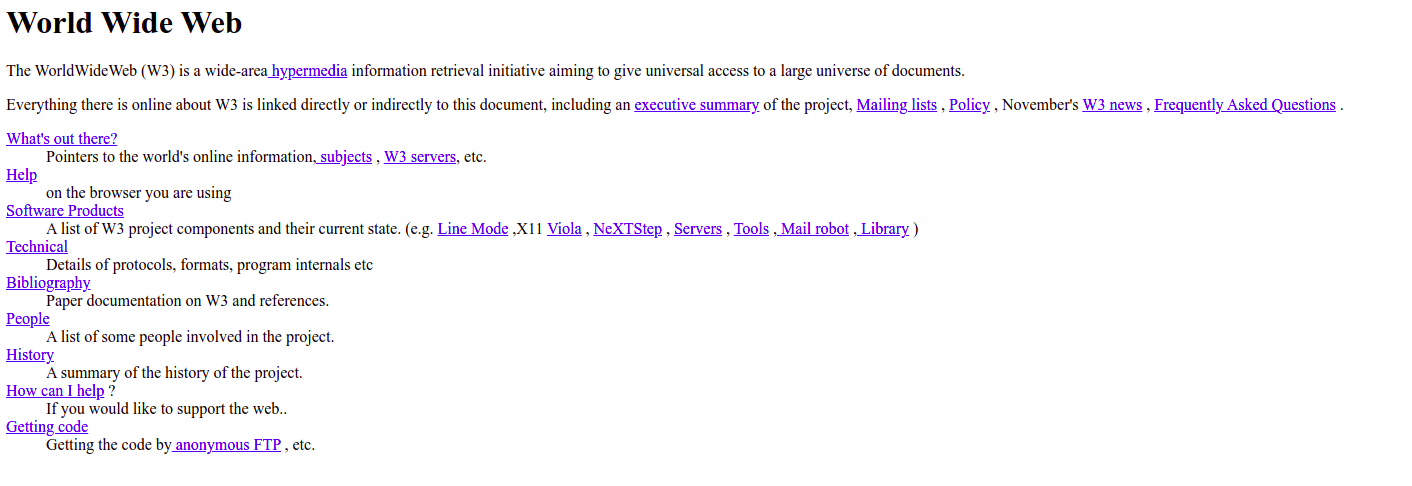
\includegraphics[width=16cm, keepaspectratio]{img/first_web_page.png}
    \caption{Primera página web}
    \label{fig:web}
\end{figure}

En la actualidad las principales ventajas de las tecnologías web son que se pueden utilizar en cualquier dispositivo, el usuario no necesita instalar nada más allá de un navegador web y su usabilidad es sencilla, si bien es necesaria una conexión a Internet para poder acceder a ellas \cite{juan}.\\

Las páginas Web modernas utilizan el modelo Cliente-Servidor, en el que el cliente hace peticiones al servidor esperando una respuesta de éste. Un mismo cliente puede estar conectado con varios servidores y a la vez interactúa con el usuario final normalmente a través de una interfaz gráfica. La parte del servidor se encarga de recibir las peticiones, analizarlas y procesarlas para enviar una respuesta. En las siguientes subsecciones, describimos algunas de las tecnologías más populares utilizadas en el desarrollo de páginas Web.

\begin{figure}[H]
    \centering
    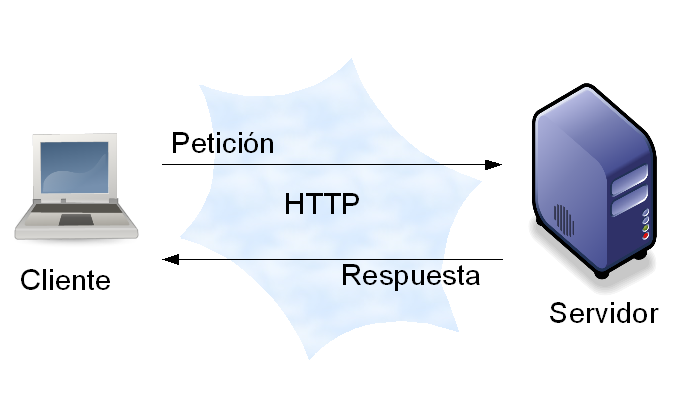
\includegraphics[width=10cm, keepaspectratio]{img/arquitectura.png}
    \caption{Arquitectura Cliente-Servidor}
    \label{fig:arquitectura}
\end{figure}

\subsection{Tecnologías web del lado del cliente}
Las tecnologías del lado del cliente suelen recibir el nombre de \textit{frontend}, son las que interactúan con el usuario, las más importantes son:

\begin{itemize}
  \item \textbf{HTML}:  Lenguaje de marcado que se encarga de dar la estructura a la página web. HTML utiliza etiquetas para mostrar los diferentes contenidos. La última versión es HTML5 donde se introducen las etiquetas de audio y vídeo.
  \item \textbf{CSS} \footnote{Cascading Style Sheets}: Lenguaje de estilo que se encarga del diseño gráfico, de la apariencia de las páginas web. La última versión es CSS3.
  \item \textbf{JavaScript}: Lenguaje de programación interpretado que permite la ejecución de código orientado a eventos (por ejemplo, pulsar un botón). Puede actuar sobre el navegador a través de objetos integrados, es decir puede manipular el HTML.
\end{itemize}

\subsection{Tecnologías web del lado del servidor}
Las tecnologías web del lado del servidor, también llamadas \textit{backend}, son las encargadas de procesar las peticiones del cliente y enviar una respuesta en forma de páginas HTML. Normalmente se utilizan \textit{frameworks }que son herramientas que te permiten desarrollar una aplicación web de forma ágil y sencilla a partir de librerías o funciones ya creadas. Algunos de estos \textit{frameworks} son:

\begin{itemize}
\item \textbf{Django}: Basado en Python. Django hace uso de plantillas permitiendo hacer páginas web más rápidas y sencillas. Gracias a su ORM \footnote{Object Relational Mapping} no es necesario saberse el manejo de base de datos ya que este traduce directamente el código de Python al lenguaje estándar de las peticiones a bases de datos, SQL.
\item \textbf{Node.js}: Permite ejecutar código JavaScript fuera del navegador y está construido con el motor de JavaScript V8 de Chrome. Node.js utiliza un modelo de entrada y salida no bloqueante, no espera a que los procesos finalicen.
\item \textbf{Symfony}: Utiliza de lenguaje de programación PHP\footnote{Hypertext Preprocessor}. Está basado en el patrón Modelo Vista Controlador (MVC). Symfony es muy flexible permitiéndote instalar únicamente lo que se necesite en vez del \textit{framework} completo.
  \item \textbf{Spring Boot}: Desarrollado para aplicaciones programadas en Java, surgió debido a que el Spring Framework era difícil de configurar. 
\item \textbf{Lavarel}: \textit{Framework} de PHP. En comparación con otros \textit{frameworks } de PHP su curva de aprendizaje es más baja. Es flexible y adaptable, no solamente debido al MVC, sino que también propone utilizar \textit{routes with clousures}, a causa de lo cual reduce código \cite{lavarel}.
\end{itemize}

%%%%%%%%%%%%%%%%%%%%%%%%%
\section{Plataforma web de programación}
En la actualidad, gracias a Internet se tiene al alcance plataformas web donde se enseña a programar de una forma interactiva. Una de las ventajas de aprender programación en una plataforma web es que puedes hacer desde la comodidad de tu casa y una gran parte son gratuitas. Pueden ser utilizadas por usuarios de todos los niveles. A continuación, se nombra algunos ejemplos de estas plataformas:\\
\newpage
\begin{itemize}
\item \textbf{Scratch}\footnote{https://scratch.mit.edu/}: Es un entorno de programación desarrollado por el MIT\footnote{Massachusetts Institute of Technology}. Se puede descargar en local o se puede utilizar la plataforma de forma \textit{online}. Utiliza un lenguaje de programación visual llamado igual que la plataforma, Scratch, el cual está basado en bloques permitiendo crear programas arrastrando y soltando para agrupar dichos bloques como un puzle. Cada bloque puede significar un evento, movimiento, un operador o una variable, entre otras. Con esta plataforma, por ejemplo, se pueden crear juegos, historias interactivas, música de manera sencilla y dinámica para el usuario. Las edades que tienen los usuarios que utilizan la plataforma esta entre los 8 y 16 años, aunque hay adultos que también la utilizan \cite{scratch}.
\end{itemize}

\begin{figure}[H]
    \centering
    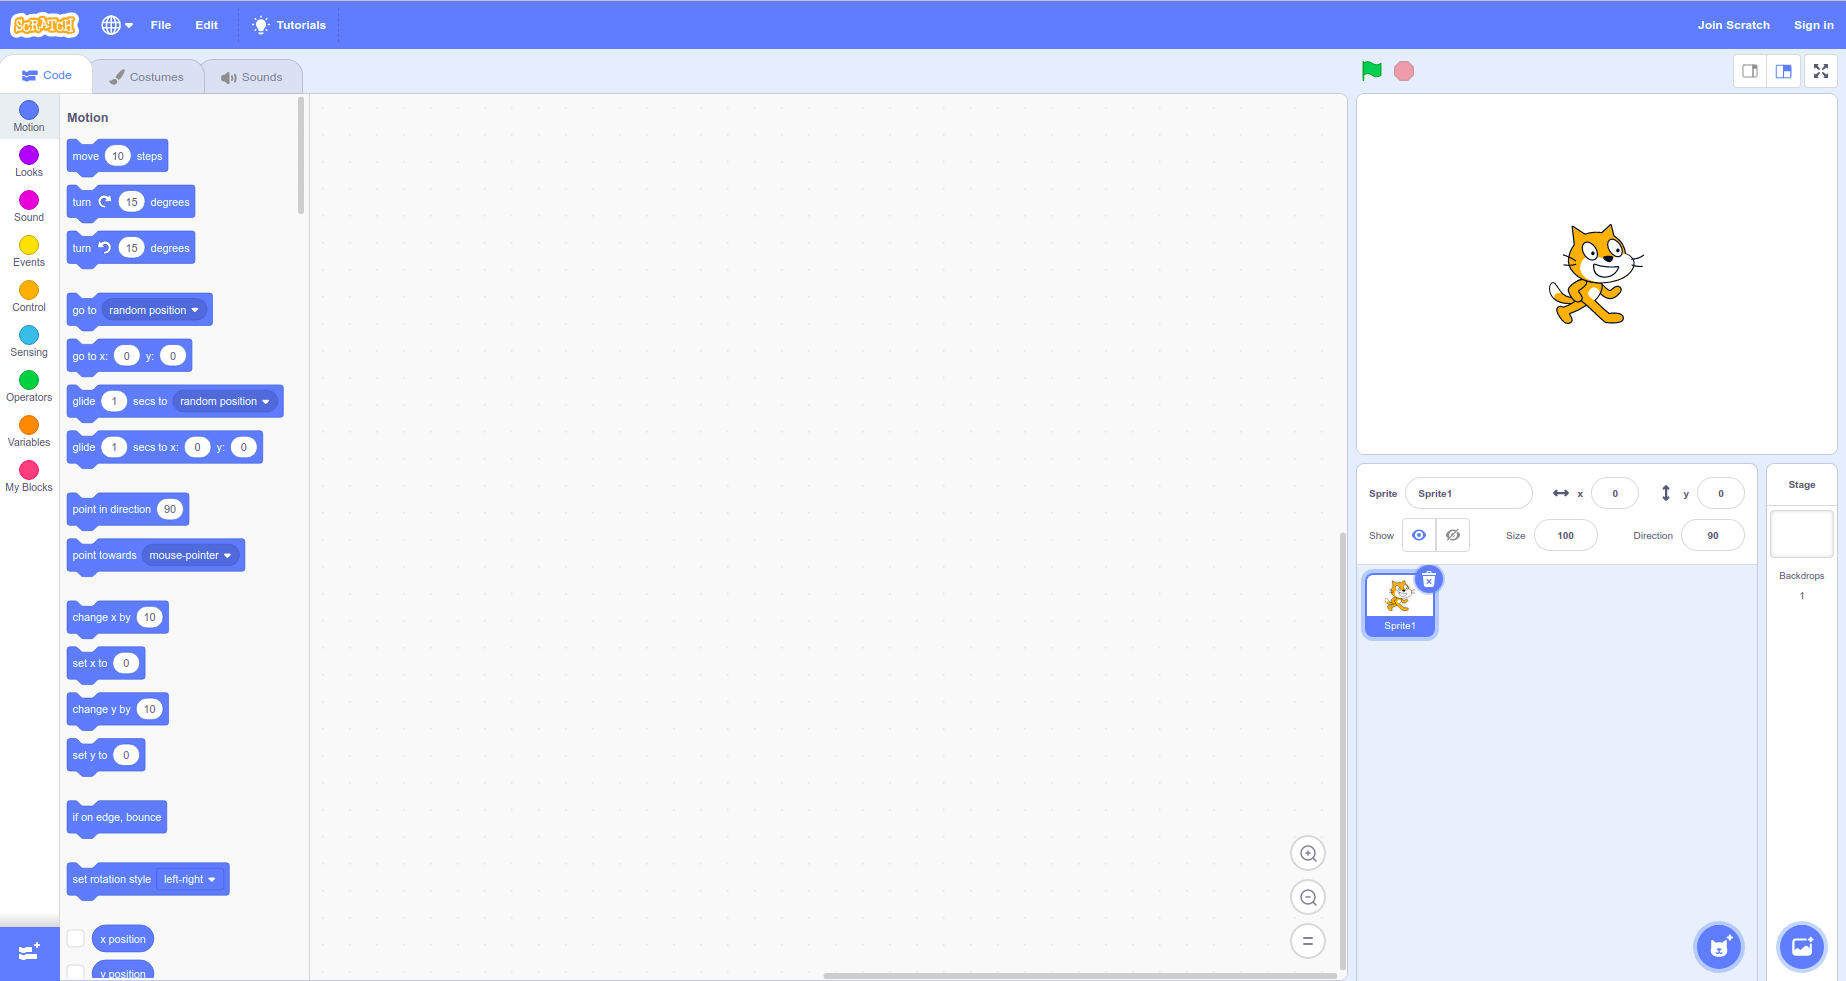
\includegraphics[width=12cm, keepaspectratio]{img/scratch.png}
    \caption{Plataforma Scratch}
    \label{fig:scrach}
\end{figure}

\begin{itemize}
\item \textbf{Snap!}\footnote{https://snap.berkeley.edu/}: Está basada en el código de programación de Scratch, creada en la Universidad de Berkeley. Esta aplicación la puedes utilizar tanto \textit{online} como descargándola y pudiendo utilizarla sin necesidad de Internet. La principal diferencia con Scratch es que te permite crear tus propios bloques utilizando JavaScript y así poder formar tu librería propia, también se puede crear listas avanzadas donde se puede almacenar cualquier tipo de dato incluso otras listas.  Esta aplicación web permite aprender a programar de una manera más visual y evitando los errores de sintaxis que se podrían cometer. Snap tiene una gran comunidad de usuarios que suben sus proyectos donde se puede aprender de ellos \cite{app}.


\begin{figure}[H]
    \centering
    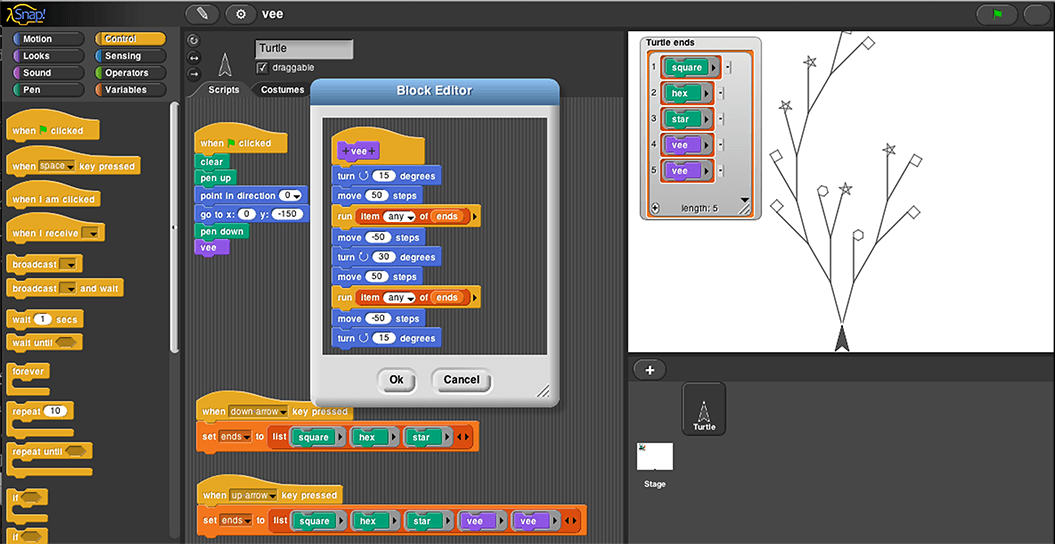
\includegraphics[width=10cm, keepaspectratio]{img/snap.png}
    \caption{Snap!}
    \label{fig:snap}
\end{figure}

\item\textbf{Robocode}\footnote{https://robocode.sourceforge.io/}: Es un videojuego multiplataforma que consiste en la creación de un tanque robot el cual tendrá que atacar y esquivar otros tanques para no ser destruido. No es necesario descargar ningún software adicional aparte del propio Robocode. Está dirigido para aprender Java y .NET. Nos podemos encontrar ligas donde las batallas de los robots transcurren en tiempo real, éstas están divididas en diferentes categorías dependiendo del tamaño de código efectivo en bytes para que sean competiciones más justas. Se puede programar las tres partes del tanque que son: el cuerpo que se encarga de mover el tanque, el radar que detecta a los adversarios y el cañón que se utiliza para apuntar y disparar. La aplicación dispone de un editor de texto, un \textit{debugger} y un compilador, todos los robots que se vayan desarrollando se podrán guardar para futuras batallas \cite{app}.


\begin{figure}[H]
    \centering
    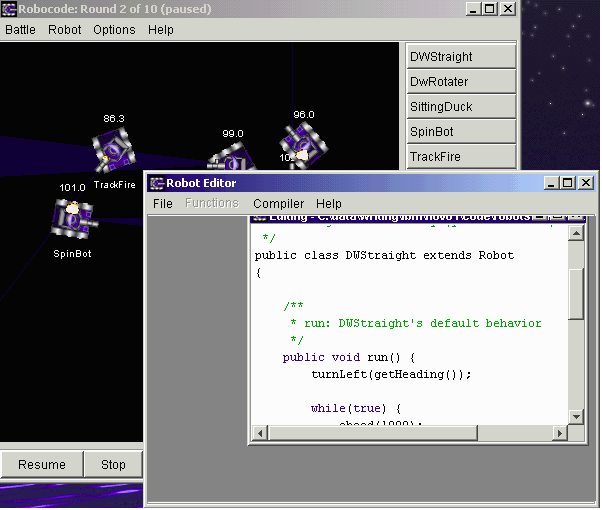
\includegraphics[width=7cm, keepaspectratio]{img/Robocode.png}
    \caption{Robocode}
    \label{fig:robocode}
\end{figure}


\item \textbf{CodeCombat}\footnote{ https://codecombat.com/}: Es una página web donde a través de un personaje se enseña a programar en diferentes lenguajes como Python, JavaScript, C++, entre otros. El objetivo del juego es ir superando los diferentes niveles, los cuales van aumentando de dificultad. Está compuesto por 110 niveles gratuitos con opción de jugar más niveles si se paga, además pagando se pueden desbloquear diferentes héroes, aprender a programar juegos y páginas web\cite{app}.
\end{itemize}

\begin{figure}[H]
    \centering
    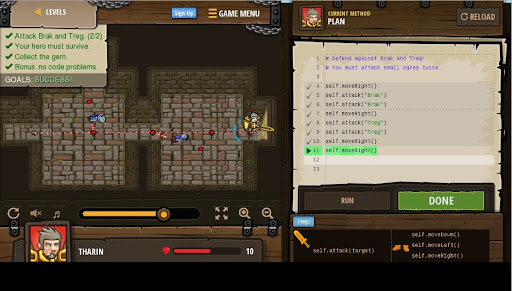
\includegraphics[width=13cm, keepaspectratio]{img/Codecombat.jpg}
    \caption{CodeCombat}
    \label{fig:codecombat}
\end{figure}

\section{Robótica y software de robot}
La robótica es la ciencia o rama tecnológica encargada del estudio, diseño, creación y aplicación de los robots. En la actualidad existen muchas formas de estudiar robótica, puedes estudiarla tanto en universidades como en cursos. Existen diferentes herramientas para poder trabajar con robots, como los sistemas operativos robóticos. Se encuentran varios ejemplos de sistemas operativos como RoboComp\footnote{https://robocomp.github.io/web/} o Player\footnote{http://playerstage.sourceforge.net/}, pero el más conocido y usado es ROS\footnote{https://www.ros.org/} (\textit{Robot Operating System}).\\

ROS es un \textit{framework} flexible para escribir \textit{software} de robots. Las principales ventajas son que es de código abierto, contando con una comunidad global para mejorar el \textit{software}. Además, es una herramienta multiplataforma e independiente de la administración del \textit{backend} y las interfaces de usuario \cite{ros}.\\

El funcionamiento de ROS está basado en nodos, éstos son procesos ejecutables que realizan una tarea simple. Las tareas de los nodos pueden ser controlar la velocidad, el motor de las ruedas o la localización. Los nodos pueden enviar mensajes o recibir mensajes de otros nodos a través de los tópicos. \\

Los tópicos se encargan de transmitir el mensaje a todos los nodos que se han suscrito y reciben los mensajes que publican los nodos. Los nodos no saben que nodo ha publicado ni que nodo se ha suscrito a un tópico. Los nodos también pueden ofrecer servicios que serán acciones que otro nodo puede pedir. El servidor que ofrece el servicio solo manda la respuesta cuando recibe una solicitud de otro nodo, haciendo la comunicación síncrona. En la Figura \ref{fig:ros} se muestra un esquema del funcionamiento de ROS \cite{ros2}.\\

Otro nodo importante es el nodo maestro que se encarga de registrar todas las suscripciones y publicaciones a los tópicos.\\

\begin{figure}[H]
    \centering
    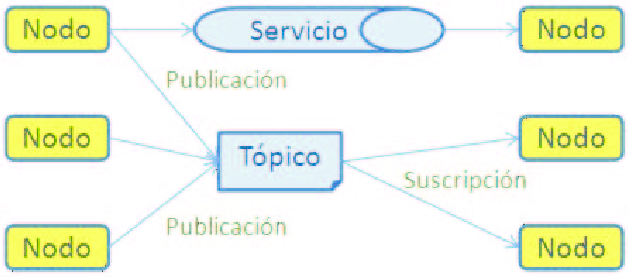
\includegraphics[width=12cm, keepaspectratio]{img/ros.png}
    \caption{Esquema ROS}
    \label{fig:ros}
\end{figure}
\newpage
Para programar robots, otra herramienta potente son los simuladores de robots. Permiten emular a robots reales de forma virtual para poder trabajar con ellos. La simulación es importante para saber cómo se comportaría un robot en la realidad y saber si necesita cambios. Además, una ventaja es que económicamente la construcción de un robot puede ser costosa, con un simulador se evitan estos gastos.\\

Existen varios simuladores como CoppeliaSim\footnote{https://www.coppeliarobotics.com/}, antiguamente llamado V-REP, cuenta con un entorno de desarrollo integrado. Cada objeto o modelo se puede controlar vía ROS, un \textit{plugin}, un \textit{script} integrado, un cliente API remoto o una solución personalizada \cite{sim}.  Webots\footnote{https://cyberbotics.com/} es otro simulador de código abierto y multiplataforma, ofrece bibliotecas con muestras de mundos, sensores o robots, entre otras características \cite{körber2021comparing}.\\

Entre todos los simuladores cabe destacar Gazebo\footnote{http://gazebosim.org/}. Para crear su simulación dinámica utiliza cuatro motores diferentes: ODE\footnote{\textit{open dynamics engine}} (simulación de cuerpos rígidos, que permite detectar y simular colisiones), Bullet (simulación de cuerpos rígidos y blandos, también detecta colisiones), DART\footnote{\textit{Dynamic Animation and Robotics Toolkit}} (simulación de la dinámica y cinemática de un robot) y Simbody (herramienta útil para simular articulaciones con restricciones y resuelve la segunda ley de Newton) \cite{upm56724}.\\

Gazebo representa gráficos 3D avanzados y realistas utilizando OGRE\footnote{\textit{Object-Oriented Graphics Rendering Engine}}, que facilita la \textit{renderización}. Dispone de diferentes sensores con la opción de añadir ruido. Además, se puede desarrollar complementos para los robots, los sensores o el ambiente. Gazebo ofrece varios robots o la posibilidad de crear uno propio \cite{gaz}.
\newpage
\section{Plataformas de programación de robótica}
Una parte de la robótica es la programación de estos robots por lo que se han ido creando herramientas de aprendizaje sencillas y atrayentes para el usuario. En Internet se pueden encontrar diversas plataformas web las cuales te enseñan sobre programación y robótica, como es el caso de Unibotics. Entre ellas se encuentran:

\begin{itemize}
\item \textbf{TheConstruct}\footnote{https://www.theconstructsim.com/}: Plataforma web que enseña sobre robótica, ROS e inteligencia artificial. Tiene una versión gratuita en la que se ofrecen tres cursos: Linux para robótica, Python3 para robótica y C++ para robótica, si se quiere puedes acceder a todos los cursos con su versión de pago. Está desarrollado para que puedan utilizarlo tanto principiantes como profesionales. No requiere de la instalación de ROS. Además, una de sus ventajas es que tiene una gran comunidad donde se puede establecer contactos y aprender nuevas formas de programar robots. TheConstruct cuenta con robots reales que se pueden alquilar por un determinado tiempo, dando la posibilidad de poder conectarse a ellos y programarlos desde cualquier lugar. Una vez se selecciona un curso, se tiene en la parte izquierda la teoría para realizar el curso. También tiene un interfaz de usuario dónde se escribe el código, un terminal para escribir comandos y una simulación del robot que se va a programar.

\begin{figure}[H]
    \centering
    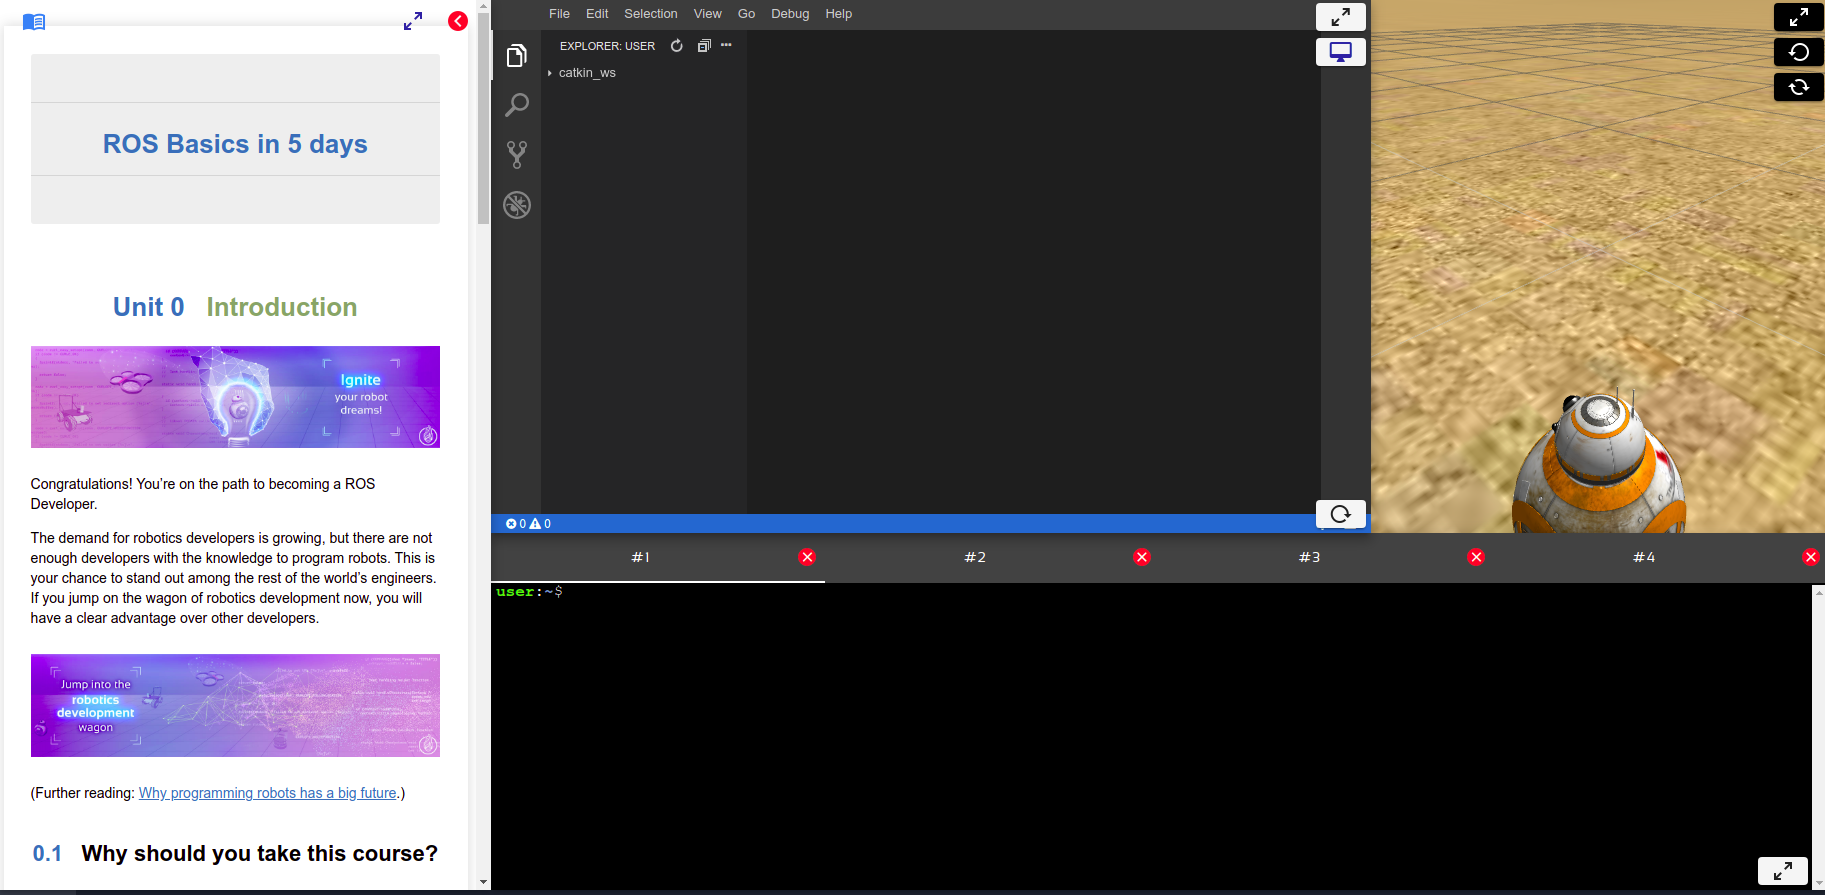
\includegraphics[width=12cm, keepaspectratio]{img/theconstruct.png}
    \caption{Curso en TheConstruct}
    \label{fig:construct}
\end{figure}
\newpage
\item \textbf{Riders.ai}\footnote{https://riders.ai/}: Plataforma robótica de simulación, educación y competencia basada en la nube, desarrollada por Acrome Robotic Systems \cite{riders}. Es una plataforma de pago, solamente es gratis la primera lección del curso Introducción a la robótica: parte 1. Consta de otros dos cursos, los cuales son la continuación del curso mencionado anteriormente. Además, una vez finalizados los cursos se obtiene un certificado. Se enseña a programar en Python o C++ los robots.  Las lecciones están formadas por la teoría, el interfaz de usuario y el simulador Gazebo, todo ello en la misma pestaña como se muestra en la figura \ref{fig:riders}.  Riders dispone de dos ligas para competir con otros programadores. Una liga consiste en drones voladores y otra sobre robots móviles.
\begin{figure}[H]
    \centering
    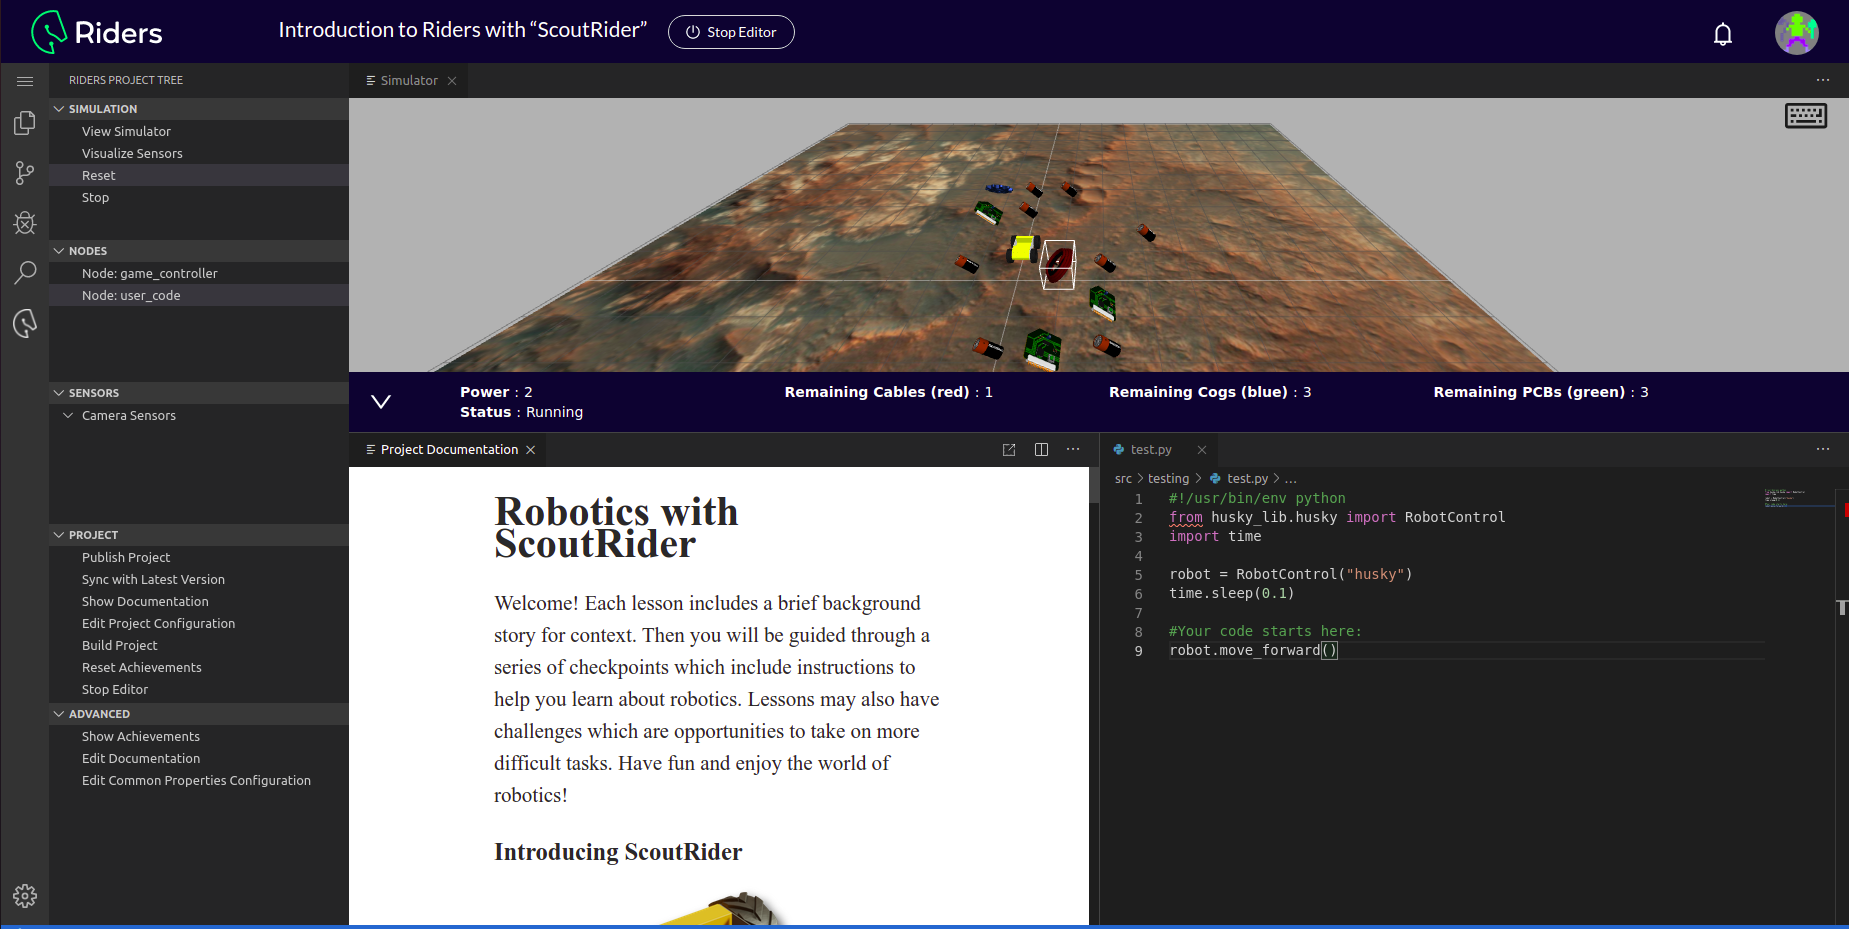
\includegraphics[width=12cm, keepaspectratio]{img/riders.png}
    \caption{Curso en Riders.ai}
    \label{fig:riders}
\end{figure}
\end{itemize}
\section{Unibotics}

Unibotics\footnote{https://unibotics.org/} es una plataforma en línea de robótica educativa donde se desarrolla este Trabajo de Fin de Grado, en la cual se enseña a programar de una manera llamativa y divertida para estudiantes universitarios. Unibotics proviene de otra plataforma que no está en línea, llamada Robotics Academy\footnote{http://jderobot.github.io/RoboticsAcademy/}. Ambas plataformas han sido creadas por la asociación de robótica e inteligencia artificial, JdeRobot.\\


La plataforma consta de varios ejercicios que se pueden dividir en ejercicios de \textbf{conducción autónoma} (\textit{Follow Line}, \textit{Obstacle avoidance}, \textit{Global Navigation}, \textit{Car Junction} y \textit{Autoparking}), \textbf{robots de servicios }(\textit{Vacuum Cleaner}, \textit{Localized Vacuum Cleaner} y \textit{Laser Mapping}), \textbf{drones} (\textit{Drone Cat and Mouse} y \textit{Rescue People}) y \textbf{visión artificial} (\textit{3D Reconstruction}, \textit{Color Filter}, \textit{OpticalFlow Teleop} y \textit{Montecarlo Visual Loc}).\\

Se puede programar los ejercicios directamente desde la web sin la necesidad de instalar software adicional. En cada ejercicio, el usuario puede introducir código fuente, cargarlo en el cerebro de un robot simulado, ejecutarlo en simulación y visualizar el interfaz gráfico. Además, se puede subir o guardar el código realizado y comprobar la eficacia y el estilo del código. Se utiliza el lenguaje Python para poder realizar los ejercicios. Unibotics utiliza una imagen de Docker llamada RADI \footnote{https://hub.docker.com/r/jderobot/robotics-academy/}(\textit{Robots Academy Docker Image} donde están preinstaladas las dependencias y así no se tiene que descargar nada localmente. Está basada en ROS y Gazebo \cite{robotics}.\\

\begin{figure}[H]
    \centering
    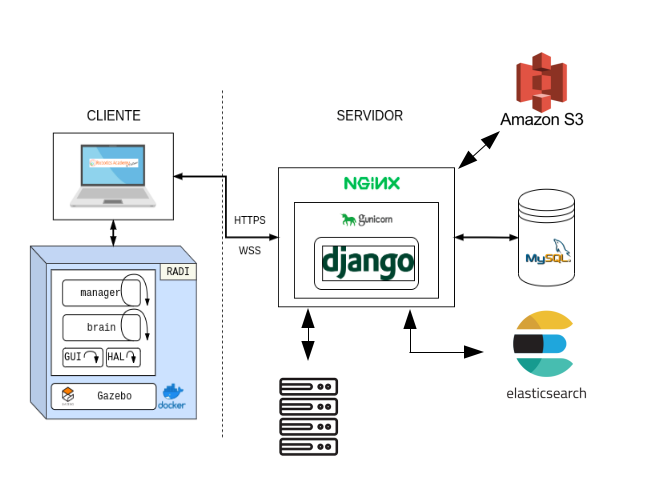
\includegraphics[width=13cm, keepaspectratio]{img/infraestructura.png}
    \caption{Infraestructura de Unibotics}
    \label{fig:infra}
\end{figure}
En la Figura \ref{fig:infra} se muestra la infraestructura de la plataforma actualmente. En la parte del servidor se encuentra un \textit{webserver}, el cual se conecta a base de datos como Elsaticsearch y MySQL, también se conecta al almacenamiento de la nube de Amazon S3 y una granja de 80 puestos. En la parte del cliente, a parte de la plataforma web se conecta a través de tres websocket al contenedor Docker, RADI. Esto hace que el coste computacional del simulador sea menor.\\

En los últimos 5 años se ha recibido ayuda de \textit{Google Summer of code}\footnote{https://summerofcode.withgoogle.com/archive/}, gracias a la cual se han ido añadiendo contenidos a la plataforma y también gracias a Trabajos de Fin de Grado.\\

En la actualidad esta plataforma es utilizada en las asignaturas de Robótica móvil y Robótica de servicios en el grado de Ingeniería de Robótica Software de la universidad Rey Juan Carlos y en el máster de visión artificial de la misma universidad.

\begin{figure}[H]
    \centering
    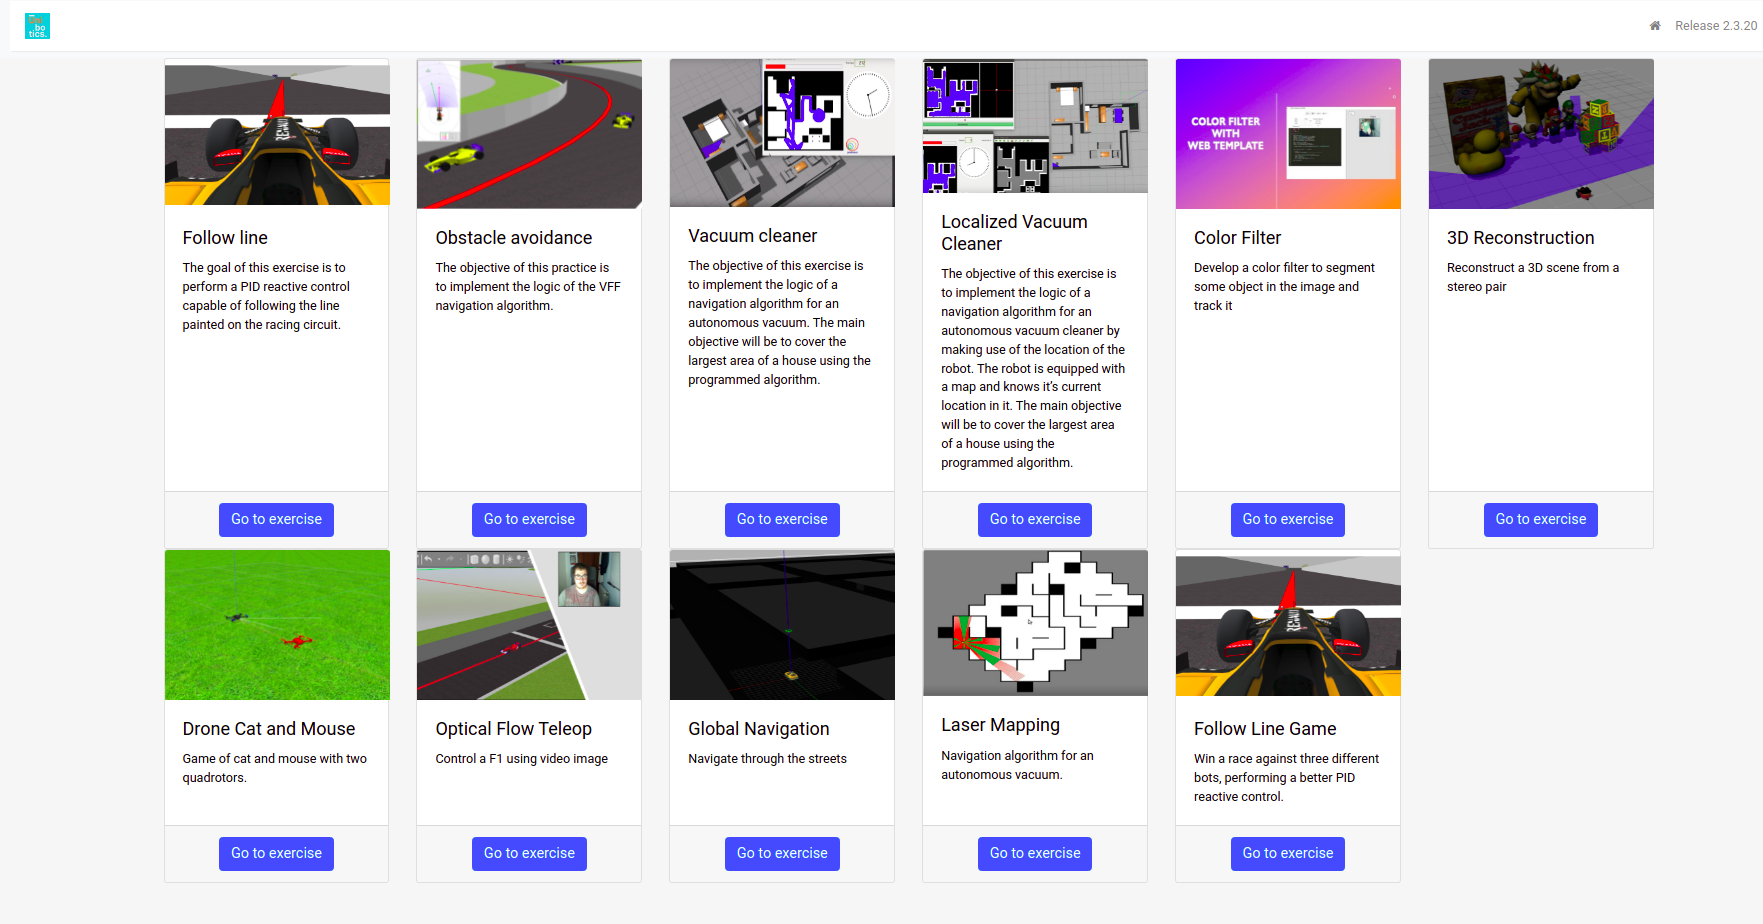
\includegraphics[width=15cm, keepaspectratio]{img/unibotics.png}
    \caption{Unibotics en la actualidad}
    \label{fig:unibotics}
\end{figure}

\section{Estructura del documento}

Este Trabajo de Fin de Grado consta de los siguientes capítulos:

\begin{itemize}
    \item \textit{Capítulo 1 Introducción}: introducción a las tecnologías web, a páginas web educativas sobre robótica y Unibotics antes de la realización de este TFG.
    \item \textit{Capítulo 2 Objetivos y Metodología}: Descripción de los diferentes objetivos a cumplir en el TFG y la metodología seguida para la realización de estos.
    \item \textit{Capítulo 3 Herramientas utilizadas}: se describen las diferentes tecnologías web utilizadas en este trabajo y las herramientas usadas para la recogida y grabación de datos y la visualización de estadísticas automáticas.
   \item \textit{Capítulo 4 Analíticas de Elasticsearch y Dash}: en este capítulo se expone el diseño y la implementación de la recogida de sondas y su posterior visualización en la plataforma de Unibotics.
  \item \textit{Capítulo 5 Conclusiones}: se desarrollan las conclusiones de los resultados obtenidos en este TFG, además de las competencias que se ha adquirido y futuros trabajos que se podrían realizar a partir de este.
   \end{itemize}

% OBJETIVOS %
%%%%%%%%%%%%%%%%%%%%%%%%%%%%%%%%%%%%%%%%%%%%%%%%%%%%%%%%%%%%%%%%%%%%%%%%%%%%%%%%
\chapter{Objetivos y Metodología del Trabajo}\label{objetivos}

En los últimos años el uso de plataformas web educativas ha ido incrementándose. La pandemia ha sido otro factor por el cual algunas clases anteriormente presenciales ahora son \textit{online}. Por consiguiente el uso de estas plataformas es más demandado. En el área robótica esto no es una excepción, y se está haciendo especial hincapié en el desarrollo de plataformas \textit{online} que permitan programar robots.\\

Para que la plataforma pueda mejorarse y ser más atrayente a los alumnos es necesario monitorizar su uso y un posterior análisis, donde los administradores podrán ver cómo los usuarios interactúan con la plataforma y tomar decisiones a partir de los resultados. Los administradores, por lo tanto, podrán ver por ejemplo cuánto tiempo los alumnos tardan en resolver un ejercicio y qué nota obtienen, pudiendo hacer correlaciones entre los datos obtenidos.\\

Para conseguir que Unibotics cuente con las mejoras mencionadas, se han establecido los siguientes objetivos, metodología y plan de trabajo.
\newpage

\section{Objetivos}

El objetivo principal que sigue este proyecto es la integración de un sistema de monitorización automática en una aplicación web,
en concreto en la plataforma web de robótica educativa
Unibotics. Para cumplir el objetivo principal se ha marcado diferentes subjetivos:

\begin{enumerate}
\item Capturar las diferentes interacciones de los usuarios, como puede ser el tiempo que un usuario está en la plataforma Unibotics. Esos datos recogidos son llamados sondas. Estas sondas serán capturadas en la parte cliente de Unibotics, utilizando JavaScript.
\item La grabación de las sondas en una base de datos.
\item Creación de gráficas dinámicas automáticas desde de las sondas recogidas. Se mostrarán en varias páginas web dentro de la propia plataforma. Por un lado, en una página de acceso exclusivo a los administradores. Por otro lado, los usuarios podrán acceder a otra página web donde ver un histórico de sus correspondientes puntuaciones en cada ejercicio.
\end{enumerate}

\section{Metodología}

La metodología seguida en este proyecto ha comenzado con la planificación de reuniones semanales con los tutores. En estas reuniones semanales se hace un repaso de lo avanzado durante toda la semana y se fijan los nuevos objetivos para la semana siguiente. Estas reuniones permitían resolver las dudas más inmediatas. Gracias a la plataforma Slack\footnote{https://slack.com/} se ha podido mantener la comunicación a lo largo de la semana y poder resolver dudas de una manera más dinámica. En el grupo creado en esta plataforma también se encontraban los administradores y otros desarrolladores de Unibotics.\\

Para hacer el seguimiento del trabajo se ha creado un blog\footnote{https://roboticslaburjc.github.io/2021-tfg-claudia-alvarez/}, donde periódicamente se han ido escribiendo los avances realizados. El blog ha sido creado con \textit{Github-Pages}\footnote{https://pages.github.com/}\\

Para comenzar el TFG se ha realizado un primer estudio del código fuente de Unibotics para entender su funcionamiento y poder comprender dónde habría que añadir el código para la recogida de las sondas. Cuando se ha fijado un objetivo semanal en el que hubiera que añadir código nuevo, lo primero se creaba una incidencia o \textit{issue} en el repositorio de Github correspondiente de Unibotics describiendo el problema, después se creaba una nueva rama o \textit{branch} en la que se trabajaba en el código que solucionaba la incidencia para no modificar directamente el código fuente original de Unibotics. Una vez conseguido solucionar la incidencia se crea un parche o \textit{pull request} con la solución donde los administradores de la plataforma lo revisan y si está todo bien fusionan la rama creada con la original.\\

Unibotics cuenta con tres despliegues: D1 se despliega en local para los desarrolladores, D2 en test para probar la plataforma antes de producción y D3 en producción, en la nube de Amazon. En este proyecto se ha trabajado principalmente en el despliegue D1.\\

Se ha seguido el modelo de desarrollo software en espiral basado en iteraciones. En cada iteración primero se establece un objetivo, la siguiente etapa es el diseño, luego la implementación y por último, la realización de pruebas.


\section{Plan de Trabajo}
El plan de trabajo que se ha diseñado consta de varias etapas:

\begin{enumerate}
\item \textbf{Estudio de Unibotics}: Estudio del código fuente de Unibotics.
\item \textbf{Estudio de los componentes de terceros y herramientas utilizadas}: Estudio de los diferentes componentes utilizados empezando por Django. Después se estudió la base de datos Elasticsearch y el visualizador Dash y por último la herramienta de contenedores \textit{docker} .\newpage
\item \textbf{Recogida y captura de sondas}: Con Elasticsearch se graban-almacenan las diferentes sondas para la monitorización de la plataforma. Además, crear una base de datos de prueba para poder trabajar en local. Incorporar las sondas que permiten recoger las principales interacciones de los usuarios con la plataforma web. Primero con un prototipo y luego sobre Unibotics.
\item \textbf{Visualización automática de las sondas}: Una vez definido qué sondas se desean capturar y añadido el código para su recogida, se crea la aplicación web para visualizarlas y poder hacer el análisis masivo.
\item \textbf{Redacción de la memoria}: Por último, se ha escrito esta memoria utilizando Latex\footnote{https://www.latex-project.org/}.
\end{enumerate}










% HERRAMIENTAS UTILIZADAS %
%%%%%%%%%%%%%%%%%%%%%%%%%%%%%%%%%%%%%%%%%%%%%%%%%%%%%%%%%%%%%%%%%%%%%%%%%%%%%%%%
\chapter{Herramientas utilizadas}
\label{herramientas}
En este capítulo se describen las tecnologías web que se han utilizado en este TFG. En Unibotics se ha utilizado como tecnologías del lado del cliente HTML para dar estructura, CSS para el diseño y JavaScript para definir las acciones. Las tecnologías del lado del servidor han sido el entorno web de Django y la base de datos MySQL\footnote{My Structured Query Language}. También se ha integrado una base de datos llamada Elasticsearch para la recogida de la información y para visualización de estadísticas automáticas se ha utilizado Dash.

\section{HTML}
HTML son las siglas de \textit{HyperText Markup Language} donde "HiperTexto" se refiere a un texto donde hay enlaces a otra página web o a la misma página permitiendo que los documentos estén interconectados entre sí. Con marcado se hace referencia a que HTML define la estructura del documento con marcas, por ejemplo, que parte del documento va a ser un título y dónde se va a encontrar. HTML es un lenguaje, pero no de programación sino de marcado.\\

La estructura de un documento HTML está compuesta por la definición del tipo de documento con \textit{\textless!DOCTYPE html\textgreater}, el elemento  \textit{\textless html\textgreater} y \textit{\textless/html\textgreater} para dar comienzo y final al documento HTML, el elemento {\textless head\textgreater} y {\textless/head\textgreater} donde se introducen los metadatos como es el idioma del documento o el título que aparece en la pestaña de la página, y el elemento {\textless body\textgreater} y {\textless/body\textgreater} donde se escribe todo el contenido que se quiere mostrar a los usuarios \cite{html}.

\begin{figure}[H]
    \centering
    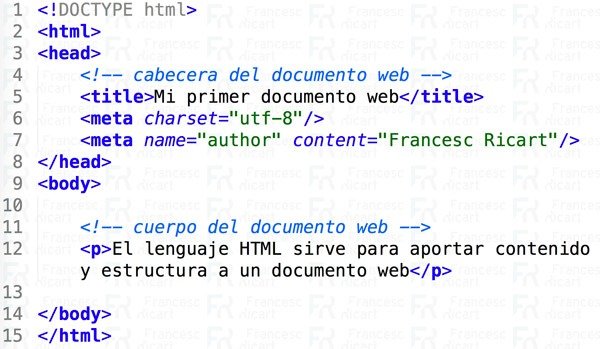
\includegraphics[width=9cm, keepaspectratio]{img/html.jpg}
    \caption{Estructura HTML}
    \label{fig:html}
\end{figure}

Un elemento de HTML está compuesto por etiquetas que son palabras que marcan el inicio y final de una sección. La etiqueta de apertura está formada por una palabra o letra rodeada por '\textless' y '\textgreater' dando comienzo al elemento y normalmente con una etiqueta de cierre al igual que la de la apertura pero rodeada por '\textless' y '\textgreater'. La etiqueta no distingue entre mayúsculas y minúsculas. Aunque haya una gran cantidad de etiquetas a veces se necesita información adicional para completar los elementos, esto se consigue gracias a los atributos.\\ 

El atributo se encuentra dentro de la etiqueta de apertura con un espacio en blanco del nombre de la etiqueta o de otro atributo, el atributo está compuesto por un nombre seguido del signo igual ( = ) y el valor del atributo entre comillas. \\

Cada etiqueta tiene unos atributos asociados y éstos a la vez unos valores predefinidos. Si se da un valor erróneo a un atributo al renderizar la página esta lo ignorará. Algunos atributos son obligatorios como en el caso de las imágenes, vídeos o enlaces, como se muestra en la Figura \ref{fig:elemento}, la etiqueta para los enlaces es \textit{a} y es obligatorio que le siga el atributo \textit{href}  para poder añadir la dirección a la que va a dirigir dicho enlace. Entre las etiquetas de apertura y cierre nos encontramos con el texto que será el contenido de la sección \cite{etiqueta}.

\begin{figure}[H]
    \centering
    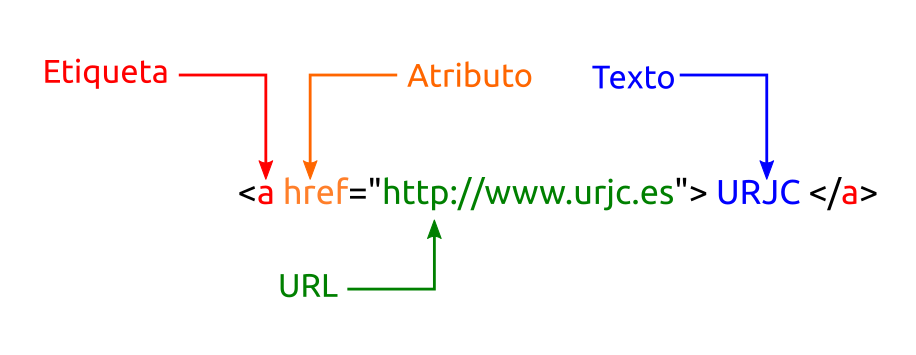
\includegraphics[width=12cm, keepaspectratio]{img/elemento.png}
    \caption{Estructura de un elemento HTML}
    \label{fig:elemento}
\end{figure}

Hay dos tipos de elementos, los bloques, que son los elementos que ocupan toda una línea en el documento estos son los encabezados, listas o párrafos; y los elementos en línea que solo ocupan el espacio de su contenido como los botones, enlaces o imágenes. Esto se puede cambiar gracias a los atributos. Para estructurar el documento disponemos de dos etiquetas generales, \textit{\textless div\textgreater} la cual crea una sección de tipo bloque y \textit{\textless span\textgreater} para crear una sección en línea \cite{juan2}.\\

La última versión del lenguaje HTML es HTML5, que ha sido la utilizada en este proyecto. Como mejoras respecto a anteriores versiones está la introducción de las etiquetas de audio \textit{\textless audio\textgreater} y vídeo \textit{\textless video\textgreater}. Anteriormente la web no estaba pensada para multimedia y había que meter parches como Flash de Adobe. En HTML5 se introduce SVG\footnote{Scalable Vector Graphics } para hacer gráficos vectoriales y así no se verán pixeladas las imágenes. También como novedad tiene Canvas, el cual es un elemento de diseño gráfico y composición de imágenes. Y WebGL, que es una especie de Canvas pero en 3D. \\

En HTML5 si el usuario del navegador da permiso, incorpora una API\footnote{Application Programming Interfaces} de geolocalización donde se puede ver la ubicación. Por último, también incorpora lo denominado \textit{Drag and Drop} que consiste en arrastrar y soltar para facilitar la interacción con el usuario.\\


\newpage
\section{CSS}
CSS es el lenguaje de estilo que se encarga del diseño y la presentación de los documentos HTML. Para llamar la atención de los usuarios en páginas web es importante añadir estilo a los documentos, por eso se utiliza CSS, el cual puede definirse como un atributo de HTML llamado \textit{style}. Otra forma de meter estilo es utilizando la etiqueta {\textless style\textgreater} en la cabeza del documento HTML. La mejor opción para añadir estilo es separándolo de la estructura, es decir, del documento HTML, creando una hoja de estilo \textit{.css}. De esta forma es más sencillo realizar cambios y se podrá diversificar el trabajo en estructura y estilo, siendo más productivo. Para vincular la hoja de estilo con el HTML se utiliza la etiqueta \textit{\textless link\textgreater} en la cabecera.\\

La estructura de una regla CSS se divide en selectores que contienen pares de propiedad-valor, como se muestra en la Figura \ref{fig:css}. En los selectores se pone el nombre de las etiquetas las cuales quieres cambiar su estilo, como puede ser la etiqueta \textit{body}. Además, estos selectores pueden ser el valor del atributo \textit{id}, que representa el identificador único. En este caso se pone el símbolo \# antes del valor de su \textit{id}. Aparte de identificar un elemento con un \textit{id} se puede utilizar el atributo \textit{class}, que es un identificador para varios elementos. En este caso para añadirle estilo a los elementos pertenecientes a la misma clase al selector se le añade un punto delante.

\begin{figure}[H]
    \centering
    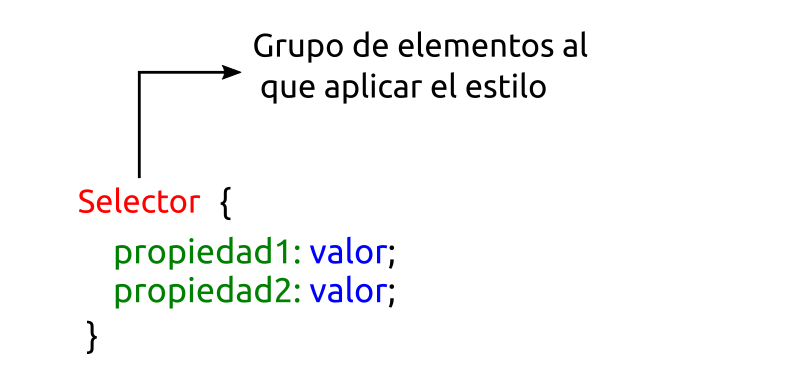
\includegraphics[width=12cm, keepaspectratio]{img/css.png}
    \caption{Sintaxis CSS}
    \label{fig:css}
\end{figure}
\newpage
Las propiedades indican cuál es el estilo que se quiere cambiar en un elemento, como puede ser el color o el tamaño. Cada propiedad tiene unos valores asociados que en algunas ocasiones se pueden escribir de diferente manera, como en el caso de los colores, se puede escribir directamente como \textit{red} o ponerlo en su valor hexadecimal o en valores RGB\footnote{ Red, Green, Blue,}.\\

A la hora de utilizar estilos se pueden poner estilos contradictorios, en este caso el último estilo definido será el que se acabe aplicando. Esta es la parte de cascada que indica las siglas CSS. Si se ha utilizado una hoja de estilo, pero además, se ha definido en una etiqueta HTML, el definido en la etiqueta será el utilizado al \textit{renderizar} el documento. La herencia también es un concepto importante en CSS ya que si un elemento no tiene estilo, pero está contenido en otro elemento que sí tiene, éste heredará su estilo. Los identificadores únicos tendrán preferencia a añadir el estilo sobre los identificadores de clase, el nombre de la etiqueta como selector es el de menor preferencia entre los selectores \cite{juan3}.


\section{JavaScript}
JavaScript es un lenguaje de programación interpretado que permite la ejecución de código orientado a eventos. Pueden actuar sobre el navegador a través de objetos integrados como un botón. El DOM\footnote{Document Object Model}, es el modelo de objetos que representa al documento HTML y define la manera de interactuar con él, puede ser modificado dinámicamente gracias a JavaScript. Es importante la colocación del código JavaScript ya que se ejecuta ordenadamente de arriba a abajo. \\

JavaScript suele estar en el lado del cliente haciendo que su código se ejecute en el navegador web, donde podrá interactuar con el navegador, además, con el documento HTML o dibujar en la página. También existen entornos para el desarrollo de la parte servidor de una plataforma Web que están basados en JavaScript, como Node.js\footnote{https://nodejs.org/} \cite{juan4}.\\
\newpage
Hay diferentes formas de agregar código JavaScript a un documento HTML. Como ocurría con CSS la mejor opción es tener un fichero .js separado de la estructura (HTML) y del estilo (CSS) para poder trabajar de una mejor manera. Para añadirlo en la cabecera del HTML se le inserta la etiqueta {\textless script\textgreater} con el atributo \textit{src} para indicar la ubicación del fichero. Para que no haya ningún problema conviene ejecutar el código cuando se haya cargado la página, para ello se utiliza el atributo \textit{onload} que indica que se ha cargado la página y se llama a una función principal del fichero JavaScript. Otra forma de introducir JavaScript en el documento HTML es directamente en sus etiquetas, por ejemplo, cuando ocurre un evento o mediante la etiqueta {\textless script\textgreater} que ofrece HTML \cite{js}.\\

En este TFG se ha utilizado JavaScript para detectar las diferentes interacciones de los usuarios en la plataforma web de Unibotics a través de eventos. También se ha hecho uso de JQuery\footnote{https://jquery.com/}, una librería de JavaScript que permite una manipulación más sencilla del DOM y de los eventos que se generan en éste. 

\section{Django}
Django es un entorno de desarrollo web de código abierto escrito en Python. Django actualmente dispone de mucha funcionalidad, es decir, viene con extras para ayudar al desarrollo de una web, además es versátil, escalable, rápido y seguro. Una de sus principales ventajas es que  levanta automáticamente una página web de administración donde se pueden hacer acciones como retocar la base de datos. Django sigue el Modelo Vista Controlador (MVC), y además incorpora plantillas como se muestra en la Figura \ref{fig:django}.\\

\begin{figure}[H]
    \centering
    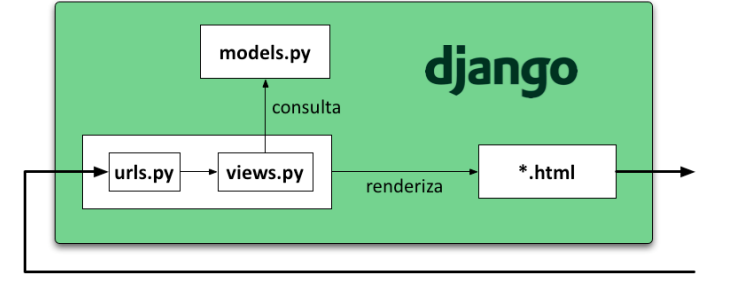
\includegraphics[width=12cm, keepaspectratio]{img/django.png}
    \caption{Estructura de Django}
    \label{fig:django}
\end{figure}

Los modelos en Django son objetos en Python que son guardados en una base de datos. Los modelos son independientes al gestor de base de datos concreta que se vaya a utilizar, se definen las estructuras de información de una manera genérica y además se puede añadir restricciones. Django puede traducir automáticamente filtros de Python en SQL gracias a su ORM, por lo tanto, no es necesario saber el lenguaje de las bases datos para hacer consultas, basta con programarlas como filtros de Python. Los modelos están formados por una lista de campos donde se define el dominio de cada campo, si no hay ningún campo que tenga una clave primaria, Django generará una columna llamada id que se incrementará automáticamente. Los modelos se escriben en el fichero \textit{models.py} \cite{model}.\\

Las vistas en Django están formadas por el fichero \textit{urls.py} y \textit{views.py}. En el fichero\textit{ urls.py} se definen a partir de expresiones regulares las urls que redirigen a funciones de \textit{views.py.} La función \textit{views.py} recibe un objeto \textit{HTTP Request} y todos los parámetros de la URL capturados teniendo que devolver un objeto \textit{HTTP Response}. Lo habitual en web dinámicas es hacer una consulta a la base de datos, generar un contexto que empotra en una plantilla y a través de la cual se \textit{renderiza} devolviendo un \textit{HTTP Response.}\\

Las plantillas son páginas dinámicas, es decir, son protopáginas las cuáles solo se pueden \textit{renderizar} juntando el contexto (diccionario con los valores que se dan a variables de la plantilla) pasado por las vistas y dando como resultado normalmente un documento HTML. Esto es útil al programar ya que permite hacer páginas dinámicas en pocas líneas\\
\newpage
En resumen, para implementar un servidor en Django primero hay que diseñar el modelo de datos, luego se diseñan las urls que enrutarán a las vistas, las cuáles preparan un contexto que juntándolo con la plantilla se genera el \textit{HTTP Response} correspondiente.\\

La versión actual de Unibotics está basada en Django 2.2.

\section{Lenguaje SQL}
SQL\footnote{Structured Query Language} es un lenguaje de consulta estructurado, se utiliza para definir, manipular y gestionar los datos almacenados en una base de datos relacional. SQL es un estándar reconocido en 1986 por ANSI\footnote{American National Standards Institute} y en 1987 por ISO\footnote{International Organization for Standardization}\\

Se necesita un gestor de base de datos RDBMS\footnote{Relational Database Management System}  que se encarga de interactuar con la base de datos, por ejemplo MySQL o  Access SQL. Algunos de estos gestores trabajan en local y otros en un servidor remoto \cite{rdbms}.\\

\begin{figure}[H]
    \centering
    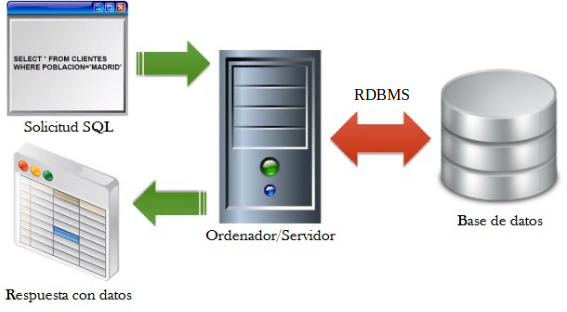
\includegraphics[width=11cm, keepaspectratio]{img/sql.png}
    \caption{Esquema funcionamiento SQL}
    \label{fig:sql}
\end{figure}
\newpage
Una instrucción SQL está formada por comandos, cláusulas, operadores y funciones. Los comandos de una sentencia SQL pueden servir para crear, modificar o hacer consultas a la base de datos, entre otras funciones.\\

Las cláusulas son condiciones de modificación para poder definir los datos que se quieren seleccionar o manipular. Entre ellas se encuentran \textit{FROM} para especificar la tabla o \textit{WHERE} para definir las condiciones de los registros que se desean.\\

Los operadores pueden ser lógicos (\textit{AND}, \textit{OR} o \textit{NOT}) o de comparación, que serían las operaciones del estilo mayor que, menor que o igual que. Las funciones se utilizan con el comando \textit{SELECT} para devolver un único valor de un grupo de registros, como puede ser\textit{ AVG }que te devuelve la media. En la Figura \ref{fig:ejsql} se muestra un ejemplo de una sentencia SQL con todas sus partes \cite{sql}.\\

\begin{figure}[H]
    \centering
    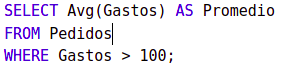
\includegraphics[width=9cm, keepaspectratio]{img/ejsql.png}
    \caption{Sentencia SQL}
    \label{fig:ejsql}
\end{figure}
En este TFG se ha utilizado SQL ya que Unibotics utiliza una base de datos MySQL donde se almacena la información estructural de la plataforma como los usuarios o los ejercicios existentes, a la cual se accede a través de Django.
\newpage
\section{Elasticsearch}
Para la recogida y grabación de las sondas es necesario tener una base de datos, en este caso para este proyecto se ha decidido utilizar una base de datos no relacional (NoSQL\footnote{\textit{Not only SQL}}). Una base de datos no relacional se caracteriza por almacenar datos no estructurados o semi-estructurados, además, sus datos no están organizados en tablas, como es el caso de las bases de datos relacionales como MySQL.\\

En este TFG se ha utilizado Elasticsearch\footnote{https://www.elastic.co/}, que es un motor de búsqueda y análisis de código abierto, escrito en Java y basado en Lucene. Asimismo, es una biblioteca de Java que proporciona funciones de indexación y búsqueda, entre otras. Elasticsearch está orientado a documentos JSON\footnote{JavaScript Object Notation}, los cuales están formados por un conjunto de pares clave-valor, donde la clave es una cadena de texto y el valor puede ser de diferentes tipos como un texto o una lista \cite{elastic}.\\

Elasticsearch se caracteriza por ser una herramienta rápida permitiendo una búsqueda de texto completo bastante eficiente. Gracias al poco tiempo transcurrido entre la indexación (grabación de datos en Elasticsearch) y la posterior búsqueda se ha considerado que es una herramienta adecuada para la grabación de las sondas de Unibotics y la posterior consulta de la información.\\

Una de las ventajas de las bases de datos no relacionales es que están implementadas para permitir un escalado horizontal, es decir se puede dividir la base de datos en diferentes servidores, de una manera más sencilla que con las bases de datos relacionales.\\

Los diferentes datos están agrupados en lo que se llama \textit{shards}, en los cuales se aplican técnicas de réplica para ser tolerante a los fallos. Además, si Elasticsearch tiene algún fallo es capaz de detectarlo y reorganizar la información. Existen diferentes módulos en diferentes lenguajes de programación que permiten una interacción sencilla con Elasticsearch \cite{elastic2}.\\

Elasticsearch está formado por \textit{clusters} que son un conjunto de nodos, en los cuales se almacenan todos los datos, también puede estar formado por un único nodo. Al \textit{cluster} se le asigna un nombre y un identificador único \cite{elastic3}.\\

Los nodos que se encuentran en un \textit{cluster} son unos servidores únicos que almacenan documentos y ayudan en las capacidades de indexación del \textit{cluster}. Al nodo también se le asigna un nombre y un identificador. Dentro de los nodos se pueden encontrar uno o más índices que son una colección de documentos con características similares, tienen que ser nombrados en minúsculas y este será el nombre al que se hará referencia para realizar las diferentes operaciones. Los documentos que se almacenan en un índice están formados por la información básica que se desea indexar \cite{elastic3}.\\



\begin{figure}[H]
    \centering
    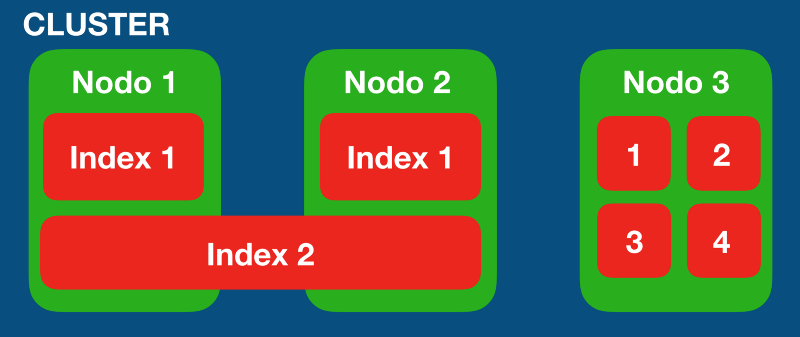
\includegraphics[width=12cm, keepaspectratio]{img/arquitectura_elastic.png}
    \caption{Arquitectura Elasticsearch}
    \label{fig:elastic}
\end{figure}
En el caso de que se guarde una gran cantidad de documentos sobrepasando los límites de almacenamiento de un nodo, Elasticsearch divide cada índice en diferentes fragmentos (\textit{shards}), la distribución de cada fragmento por los diferentes nodos se realiza de forma automática. Para evitar fallos en los nodos se hacen réplicas de los \textit{shards} y se almacenan en un nodo diferente al \textit{shard} primario. Así en el caso de que se produzca un fallo en un nodo se podrá seguir trabajando.\\

En este TFG se ha utilizado la versión 7.12.0 de Elasticsearch.


\section{DASH}

En este TFG se ha decidido utilizar el entorno Dash\footnote{https://dash.plotly.com/} para visualizar los datos recogidos. Dash es un \textit{low-code framework}, es decir que permite la creación de aplicaciones de manera rápida y eficiente haciendo un menor uso de la programación manual, está escrito sobre Plotly.js y React.js. Dash está disponible en lenguajes de programación como Python, Julia, R o F#. Dash es multiplataforma, por lo que puede ser utilizado desde cualquier dispositivo \cite{dash}.\\

En las aplicaciones de Dash no es necesario escribir ningún documento HTML, JavaScript o CSS ya que Dash proporciona una abstracción pura en Python mediante el uso de la biblioteca de \texttt{dash\_html\_components}. Otra biblioteca de Python que se utiliza en una aplicación Dash es \texttt{dash-core-components} la cual incluye una serie de componentes para una interfaz de usuario interactiva, como un menú desplegable.\\

La estructura de los datos que se van a visualizar en  Dash son \textit{dataframes} de la biblioteca de Pandas\footnote{Python Data Analysis Library}. Un \textit{dataframe} es una tabla en la que los datos guardados en cada columna representan las diferentes variables.\\

Las aplicaciones de Dash están formadas por dos partes. La primera es la llamada \textit{layout} donde se describe cuál va a ser el aspecto de la aplicación, esto son los menús y las gráficas que se visualizan, aquí es donde se utilizaran las bibliotecas mencionadas anteriormente. La segunda parte es la interactividad con los usuarios, para ello se utiliza \texttt{dash.dependencies} donde los componentes interactivos crean una entrada y a través de \textit{callbacks} modifican las gráficas, de tal manera que se pueden integrar filtros para generar diferentes visualizaciones en base a las necesidades del usuario.\\

Para este TFG se ha utilizado la versión 1.17.0 de Dash.

















% ANALÍTICAS DE ELASTICSEARCH Y DASH%
%%%%%%%%%%%%%%%%%%%%%%%%%%%%%%%%%%%%%%%%%%%%%%%%%%%%%%%%%%%%%%%%%%%%%%%%%%%%%%%%
\chapter{Analíticas automáticas en Unibotics}
\label{analiticas}
En este capítulo se explica la recogida de las sondas en Unibotics, su posterior guardado en la base de datos Elasticsearch, la visualización de dichos datos con el \textit{framework} web Dash y la validación experimental del proceso.

\section{Diseño}
Para conseguir las analíticas automáticas en Unibotics, se ha hecho un diseño de los cambios en la plataforma con las nuevas tecnologías involucradas: Elasticsearch y Dash.\\

\begin{figure}[H]
    \centering
    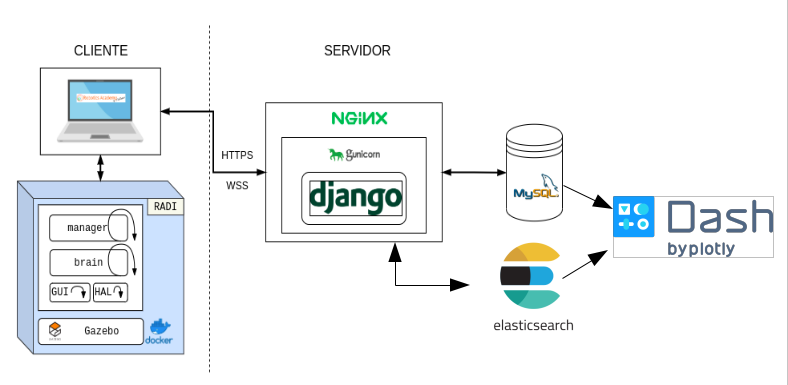
\includegraphics[width=10cm, keepaspectratio]{img/grafico.png}
    \caption{Antigua arquitectura de Unibotics}
    \label{fig:grafico}
\end{figure}

En la Figura \ref{fig:grafico} se presenta la arquitectura de Unibotics. Como se describe en la sección 1.5, Unibotics esta formado por un \textit{frontend}, dónde se encuentra el cliente conectado a un contenedor RADI que tiene el simulador. La parte del \textit{backend}
está compuesta por Django, el cual se conecta a la base de datos MySQL y a la nube de Amazon, S3.

\begin{figure}[H]
    \centering
    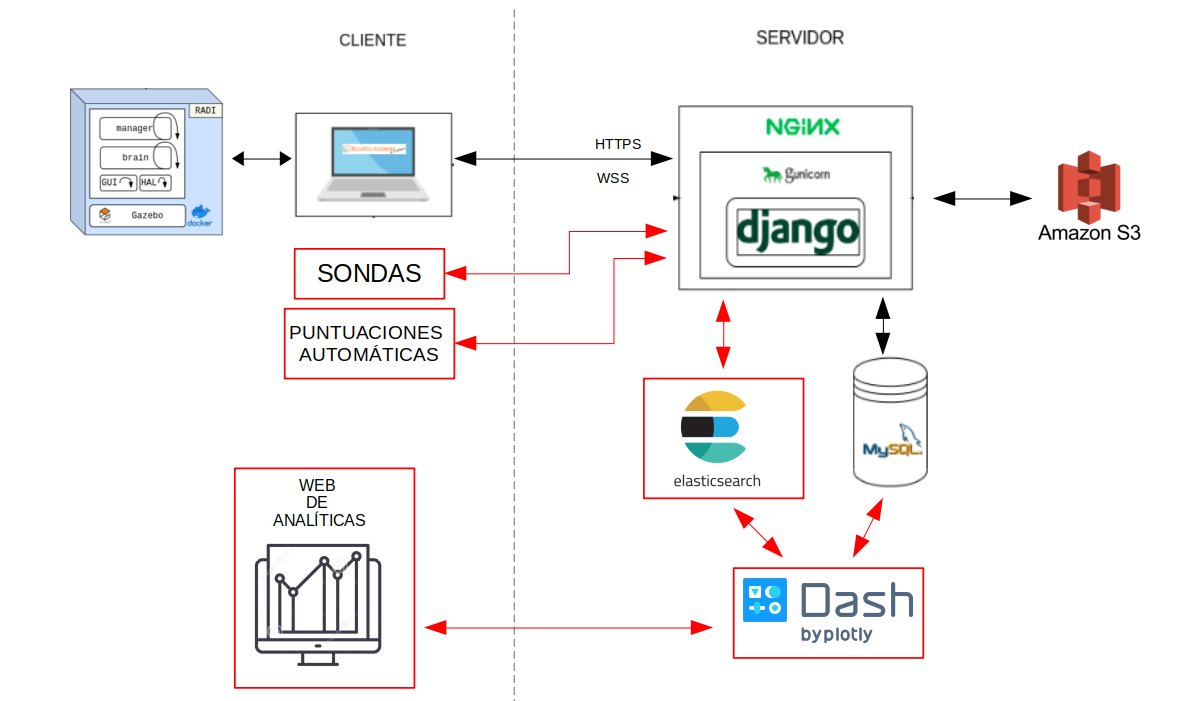
\includegraphics[width=15cm, keepaspectratio]{img/grafico2.png}
    \caption{Arquitectura Unibotics con las nuevas tecnologías}
    \label{fig:grafico2}
\end{figure}
La Figura \ref{fig:grafico2}  muestra como es la arquitectura de Unibotics, después de este TFG. En la parte del \textit{frontend}, se ha añadido la recogida de sondas con código JavaScript, al igual que las puntuaciones automáticas. Además está la web de analíticas dónde se ven las gráficas. Por otro lado, en el \textit{backend}, se ha añadido la base de datos Elasticsearch y la herramienta de Dash para las visualizaciones.\\

Lo primero que hace un usuario cuando quiere entrar en la plataforma es registrarse en ella, guardando ese registro en la base de datos MySQL. Una vez registrado, podrá iniciar sesión en ella, en el momento que desee. Cuando se encuentre dentro de la plataforma, podrá elegir un ejercicio y acceder a él, dónde podrá programar la solución. Dentro de los ejercicios tienen la opción de pedir una evaluación automática de estilo y eficacia del código programado. Para abandonar la plataforma se puede cerrar sesión o de manera implícita, cerrando el navegador o la pestaña.\\

Cuando un usuario interactúa con la plataforma de Unibotics, la herramienta de Elasticsearch recoge la información de éste. Las visualizaciones de las sondas recogidas se hacen a través de Dash, herramienta independiente a Django. Dash utiliza la base de datos de MySQL y Elasticsearch.\\
\section{Recogida de sondas}
La primera parte de este proceso ha consistido en la recogida de diferentes sondas. Para realizar esta tarea, se ha decidido utilizar la herramienta de Elasticsearch por las ventajas que ofrece explicadas en el capítulo 3.\\

En este proyecto se ha utilizado la imagen de Docker de Elasticsearch debido a que permite que funcione en cualquier sistema operativo y replicar la instalación en cualquier máquina es directo. Primero hay que descargar la imagen de Elasticsearch con la versión deseada en este caso se ha utilizado la 7.12.0, el comando para descargar la imagen es:
{\footnotesize
		\begin{verbatim}
			docker pull docker.elastic.co/elasticsearch/elasticsearch:7.12.0
		\end{verbatim}
		}
        
Para ejecutar el contenedor con la imagen descargada se utiliza el siguiente comando:

{\footnotesize
		\begin{verbatim}
			docker run --name=AcademyElastic -p 9200:9200 -p 9300:9300
            -e "discovery.type=single-node" 
            docker.elastic.co/elasticsearch/elasticsearch:7.12.0
		\end{verbatim}
		}
\newpage
  Una vez puesto en marcha el contenedor de Elasticsearch, se tiene la base de datos donde se guardarán las sondas. Es posible realizar solicitudes directamente desde el navegador web accediendo a la URL dónde esté desplegada la base de datos, por ejemplo: \texttt{http://localhost:9200/}.\\
  
  El siguiente paso es la integración de Elasticsearch en el servidor basado en Django. Para ello se hará uso de la librería \texttt{django-elasticsearch-dsl}. Además, se ha modificado el archivo de configuración del proyecto, \texttt{settings.py}. Se ha incluido la librería a las aplicaciones instaladas y creado una nueva variable, llamada \texttt{ELASTICSEARCH\_DSL}. Se ha añadido en \texttt{settings.py}, ya que las variables declaradas en ese fichero se pueden utilizar en cualquier parte del servidor. En esa variable se indica cual es el servidor de Elasticsearch, con el que se tiene que conectar y sincronizar.\\
  
Una vez conectado Django con Elasticsearch se han definido y configurado los índices donde se guardarán las sondas. Para ello, se ha creado un nuevo archivo, llamado \texttt{probe.py}. Al definir un índice, se determinan los nombres de cada campo (información que se quiere almacenar) con el tipo de campo que es, por ejemplo: un texto, un número, una fecha, entre otros. También, se puede configurar el índice, por ejemplo, poniendo el número de\textit{ shards }o el número de réplicas. Un ejemplo de la definición de un índice sería este: 

\begin{lstlisting}
   from django_elasticsearch_dsl import Document, Date, Text, Double
   
   class SessionDocument(Document):
    		username = Text()
  	  		start_date = Date()
   			end_date = Date()
    		duration = Double()
    		client_ip = Text()
    		browser = Text()
    		country = Text()
    		alpha_2 = Text()
    		alpha_3 = Text()
    		continent = Text()
    		class Index:
        		name = 'session_log'
        		settings = {
            			'number_of_shards': 1,
           				'number_of_replicas': 0
        }
\end{lstlisting} 

Para este proyecto se han definido cuatro índices diferentes:

\begin{itemize}
\item \texttt{session\_log}: índice que recoge las sondas relativas a las sesiones. Consta de los campos de inicio y fin de sesión, duración de la sesión, la IP, el \textit{browser} (aporta información sobre el sistema operativo, navegador y dispositivo utilizado), el continente y país del usuario, así como el nombre del usuario.
\item \texttt{exercises\_log}: índice que recoge las sondas relativas a los diferentes ejercicios. Está compuesto por la fecha de entrada en un ejercicio, la fecha de salida del ejercicio, la duración total, el nombre del ejercicio y el usuario.
\item \texttt{style\_log}: índice que recoge los datos sobre la evaluación del estilo del código de los ejercicios. Este índice está formado por el campo de la fecha en la que se realiza la evaluación, el nombre del ejercicio, la puntuación sobre 100 y el nombre del usuario.
\item \texttt{efficacy\_log}: índice que recoge los datos sobre la evaluación de la eficacia del código de los ejercicios. Los campos son iguales que en el índice de \texttt{style\_log}.
\end{itemize}

Ya definidos los diferentes índices, se importan al archivo \texttt{views.py} para poder crearlos. Las sesiones de los usuarios se guardan en el índice \texttt{session\_log}. A través de las sondas creadas, podemos recoger cuando el usuario \textit{loguea} en la plataforma y cuando finaliza su actividad en ella. Se recoge la sonda de la siguiente manera:
\\
{\footnotesize
\begin{verbatim}
    probe_session = SessionDocument(username=username,start_date=datetime.now(),
                                    end_date=datetime.now(),duration=0, client_ip=ip,
                                    browser=request.META['HTTP_USER_AGENT'],
                                    country=location_info["country_name"],
                                    alpha_2=location_info["alpha_2"], 
                                    alpha_3=location_info["alpha_3"],
                                    continent=location_info["continent"])
    probe_session.save()
\end{verbatim}
}
\newpage
Gracias al objeto HTTP Request que recibe el fichero \texttt{views.py}, se obtiene la información del nombre del usuario, la IP y el \textit{user-agent}. En el \textit{user-agent} se encuentra el sistema operativo, el navegador o el dispositivo que utiliza el usuario. Para la localización se ha creado una función que, a partir de la IP, muestra la ubicación. Cuando el usuario \textit{loguea}, los campos de fin de sesión y duración se inicializan con la fecha actual y 0 respectivamente, una vez que el usuario haga \textit{logout} o finalice su sesión por inactividad estos campos se modificarán como se muestra a continuación:\\
{\footnotesize
\begin{verbatim}
    s = Search(index="session_log").query('match', username=request.user.username) \
                                    .sort({"start_date": {'order':'desc'}})[0]
    for hit in s:
        end = datetime.now()
        Elasticsearch(settings.ELASTICSEARCH_DSL['default']['hosts']) \
                        .update(index="session_log", id=hit.meta.id,
                                body={"doc": {'end_date': end,
                                'duration':(end - datetime \
                                    .strptime(hit.start_date,'%Y%m%dT%H:%M:%S.%f')) \
                                    .total_seconds()}})
\end{verbatim}
}
\\
Las sondas relativas a los ejercicios se guardan cuando el usuario accede a un ejercicio. Como ocurre con las sesiones, cuando el usuario abandone el ejercicio se modificarán los datos de duración y fin del ejercicio. Se ha tenido en cuenta que al recargar un ejercicio en el que el usuario ya se encontraba, no se cree una sonda nueva y se tenga en cuenta la primera sonda creada para dicho ejercicio. Las sondas no deseadas que se han creado se eliminan de la siguiente forma:\\
\\
{\footnotesize
\begin{verbatim}
   es = Search(index="exercises_log").query('match', duration=0)  \
   				            .query('match', username=request.user.username)  \
        					                .sort({"start_date": {'order':'desc'}})
    for hit in es:
        Elasticsearch(settings.ELASTICSEARCH_DSL['default']['hosts'])  \ 
    				                        .delete(index="exercises_log", id=hit.meta.id)
\end{verbatim}
}
\newpage
Cada ejercicio que se encuentra en Unibotics dispone de un botón de evaluación automática de estilo, donde se dan unas recomendaciones para mejorar el estilo del código del usuario y una puntuación. La puntuación es recogida en el índice de \texttt{style\_log}. Para poder recoger la puntuación recibida en la evaluación de eficacia, se ha creado un nuevo botón en los ejercicios. Una vez pulsado el botón, empieza a ejecutar el código durante un tiempo determinado, según el ejercicio. Pasado ese tiempo se obtiene la nota obtenida del ejercicio y se guarda en el índice de \texttt{efficacy\_log}. Si el usuario pulsa dos veces al botón, se considera que el usuario no desea la evaluación automática, por lo cual la sonda no se guardará.\\


En este proceso de recogida de sondas y su grabación ha sido muy útil la utilización de la API que proporciona Elasticsearch para poder depurar y comprobar los datos que se estaban almacenando. Utilizando por ejemplo la URL    \newline       \texttt{http://127.0.0.1:9200/session\_log/\_search/?size=10000&pretty}, se comprueba las sondas de sesiones.\\

Las sondas recogidas han estado en producción desde el 5 de mayo de 2021. Como resultado, se ha obtenido la información de usuarios reales desde esa fecha.\\

Para comprobar el funcionamiento de Elasticsearch se generaron datos de prueba para poder comenzar a trabajar antes de tener los datos reales, los cuales llevan tiempo recoger. La base de datos Elasticsearch dummy se ha creado gracias a las librerías de Python Faker\footnote{https://faker.readthedocs.io/en/master/} y Tornado\footnote{https://www.tornadoweb.org/en/stable/} en ella se puede modificar las sondas. Por ejemplo, el número de sondas, de réplicas o de \textit{shards}. Esto ayudará a futuros desarrolladores a utilizar la base de datos de Elasticsearch. En la Figura\ref{fig:dummy} se muestra el resultado de la sonda de evaluación de estilo de la base de datos de prueba.


\begin{figure}[H]
    \centering
    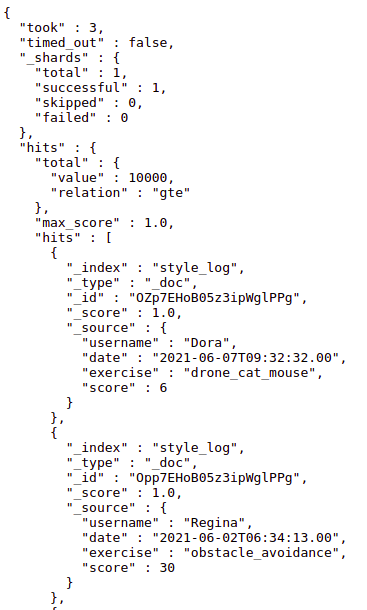
\includegraphics[width=6cm, keepaspectratio]{img/dummy.png}
    \caption{Elasticsearch dummy}
    \label{fig:dummy}
\end{figure}

\section{Visualización de la información}

Dash es un \textit{framework} web que permite crear tableros web interactivos con visualizaciones dinámicas, para poder hacer análisis como se explica en el capítulo 3. En este Trabajo de fin de grado se ha decidido utilizar esta herramienta para la visualización de las sondas recogidas en Elasticsearch.\\

Solo los usuarios registrados en Unibotics podrán acceder a las visualizaciones. Dependiendo del tipo de usuario, se tiene disponible unas visualizaciones u otras. Para iniciar sesión, se ha hecho uso de los usuarios ya guardados en la base de datos MySQL de la que depende Django, en la que se encuentra la información sobre el tipo de usuario (\textit{staff}, \textit{admin}, \textit{user}...). En el caso de los administradores podrán ver la información de todas las sondas, mientras que un usuario de Unibotics solo podrá acceder a las puntuaciones de estilo y de eficacia obtenidas en cada ejercicio. En la Figura \ref{fig:menu} muestra el menú disponible para los administradores.

\begin{figure}[H]
    \centering
    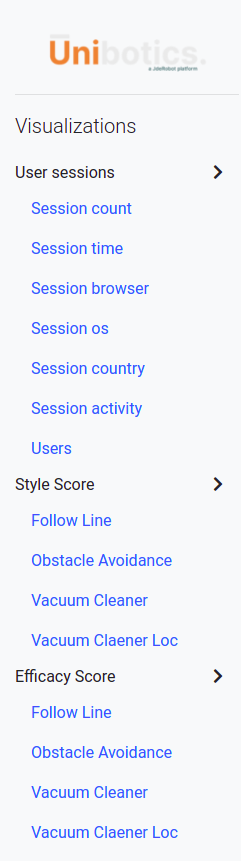
\includegraphics[width=3cm, keepaspectratio]{img/menu.png}
    \caption{Menú de un administrador en Dash}
    \label{fig:menu}
\end{figure}


Gracias a las bibliotecas de Dash, mencionadas en el capítulo 3, se ha dado estilo y formato a la aplicación. También, se ha hecho uso de las \textit{cookies }del navegador, guardadas al inicio de sesión de Dash, para comprobar si se está autorizado y si es un administrador de la plataforma.\\

Dash trabaja con dataframes, por lo que es necesario realizar una primera transformación de los datos de Elasticsearch a esta estructura, gracias a la biblioteca de Pandas. Un ejemplo de la realización de esta conversión es:

{\footnotesize
\begin{verbatim}
  s = Search(using=es, index="session_log")
  results = [hit.to_dict() for hit in s.scan()]
  df  = pd.DataFrame(results)
\end{verbatim}
}
\\
\\
Con la biblioteca \texttt{dash\_core\_components} se han creado los filtros que algunas de las gráficas poseen. Estos filtros de forma dinámica, cambian las visualizaciones en base a dicho filtrado. Uno de los filtros que más se ha utilizado es el filtro por fechas. Estableciendo una fecha de inicio o de fin o ambas. Es posible conocer la situación de Unibotics en un periodo de tiempo concreto. El código de filtrado es:

{\footnotesize
\begin{verbatim}
 if start_date is not None and end_date is not None:
        df=df.loc[(df['start_date'] > start_date) & (df['start_date'] <= end_date)]
elif start_date is not None:
        df=df.loc[(df['start_date'] > start_date)]
elif end_date is not None:
        df=df.loc[(df['start_date'] <= end_date)]
\end{verbatim}
}
\\

Otro filtro recurrente en la mayoría de las visualizaciones es el filtro por usuario. Este filtro solo aparece en las gráficas accesibles por los administradores, de forma que se puedan visualizar los datos de los diferentes usuarios de la plataforma. Para este filtro se hace uso de las sondas de sesiones, recogiendo los nombres de los usuarios de forma única y añadiendo un 'Total' en los casos que se quiera visualizar las sondas de todos los usuarios. En resumen, el filtro podrá filtrar por usuario único, un grupo de usuarios o por el total de los usuarios, \newline\texttt{df = df[df.username.isin(user)]} . El código para conseguir los nombres de los usuarios y añadir la opción de 'Total', es el siguiente:

{\footnotesize
\begin{verbatim}
	s = Search(using=es, index="session_log")
    results = [hit.to_dict() for hit in s.scan()]
    df  = pd.DataFrame(results)
    df = df[df['username'].notna()]
    users = df['username'].unique()
    if not exercises:
        users = np.insert(users,0,'Total')
    return users
\end{verbatim}
}
\\
\begin{figure}[H]
    \centering
    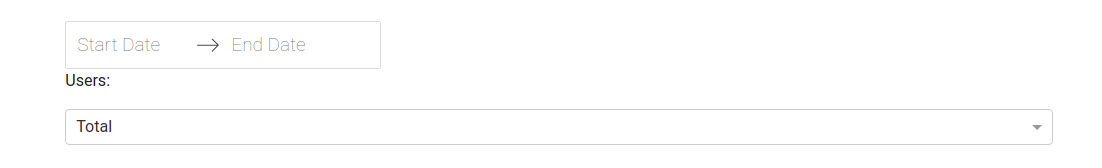
\includegraphics[width=16cm, keepaspectratio]{img/filtros.png}
    \caption{Filtros utilizados en Dash}
    \label{fig:filtros}
\end{figure}

Dash utiliza el módulo Plotly para generar las visualizaciones. Plotly ofrece una gran variedad de gráficas que se pueden utilizar en Dash. Adicionalmente se puede combinar varias gráficas en los mismos ejes, haciendo más sencilla la correlación entre datos.\\

\\
En las siguientes subsecciones, se detallan los resultados finales de las analíticas con datos reales de la plataforma de Unibotics. Se muestran las diferentes gráficas creadas tanto para administradores como para los usuarios, así como una explicación de lo que representan.
\subsection{Registros y usuarios de la plataforma}
Los administradores tienen la opción de poder ver el número total de usuarios que son activos, el número de usuarios que han sido activos en los últimos 2 meses, en formato numérico. Además, se muestra las gráficas de línea de registros por cada día, registros acumulados por días (Figura \ref{fig:accumulated}) y usuarios activos en los últimos 2 meses (Figura \ref{fig:active}). Cada una de estas gráficas contiene su propio filtrado por fechas.\\

Para la gráfica de usuarios activos, empezando por la primera sesión recogida en
\texttt{session\_log} hasta el día actual, se comprueba cuantos usuarios han iniciado sesión desde 2 meses atrás hasta el día que se está comprobando. El código para crear una gráfica de línea es el siguiente, en este caso del número de usuarios activos por día:
\begin{verbatim}
def get_temporal_figure_active_users(df):
    fig = px.line(df, x='Date', y='Active Users')
    fig.add_trace(go.Scatter(x=df["Date"].tolist(), 
                             y=df["Active Users"].tolist(),
                             mode="markers", textposition="top center", 
                             name="Active Users",
                             text=df["Active Users"].tolist()))
return fig
\end{verbatim}
\\
Las gráficas de las Figuras \ref{fig:users} y \ref{fig:accumulated} han sido elaboradas con la base de datos MySQL. Se ha realizado una lista de todas las fechas de los registros en Unibotics. Esta lista se ha convertido en dataframes. Se ha contado el número de repeticiones de cada fecha y su acumulación, dando como resultado dichas gráficas.\\



\begin{figure}[H]
    \centering
    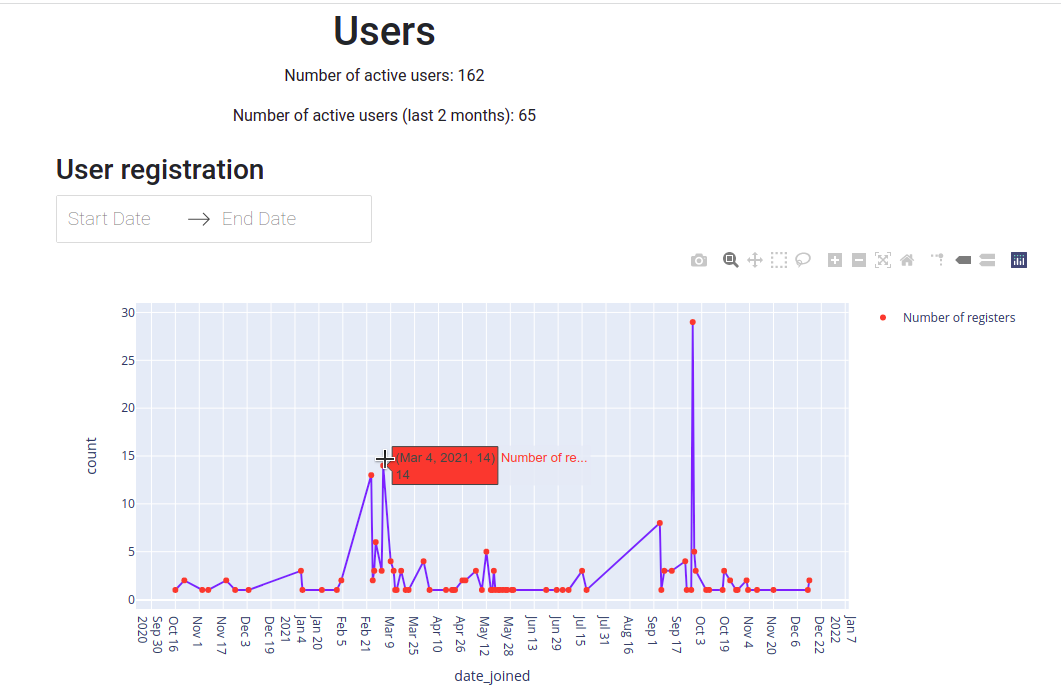
\includegraphics[width=16cm, keepaspectratio]{img/users.png}
    \caption{Gráficas relativas a los usuarios}
    \label{fig:users}
\end{figure}
\begin{figure}[H]
    \centering
    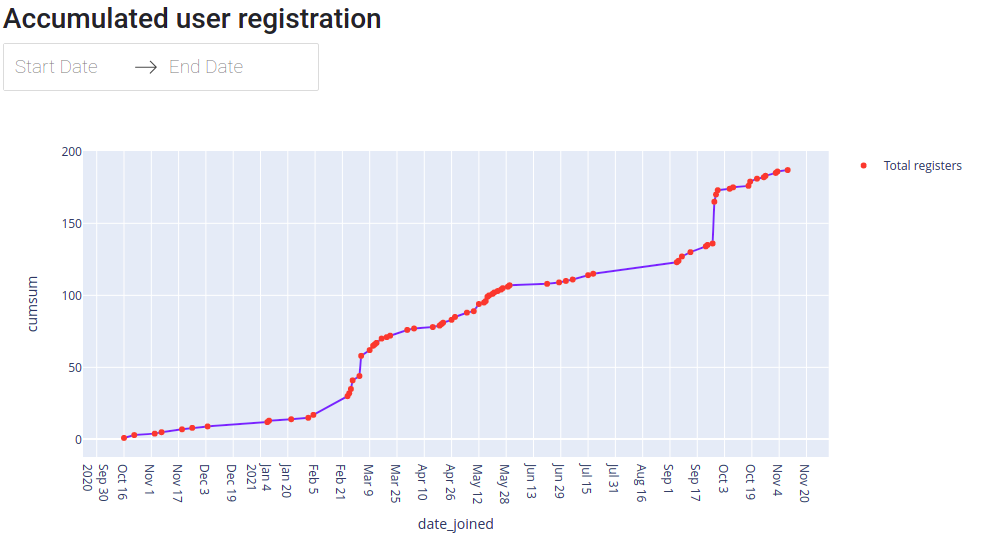
\includegraphics[width=16cm, keepaspectratio]{img/accumulated.png}
    \caption{Gráfica registro de usuarios acumulado}
    \label{fig:accumulated}
\end{figure}
\begin{figure}[H]
    \centering
    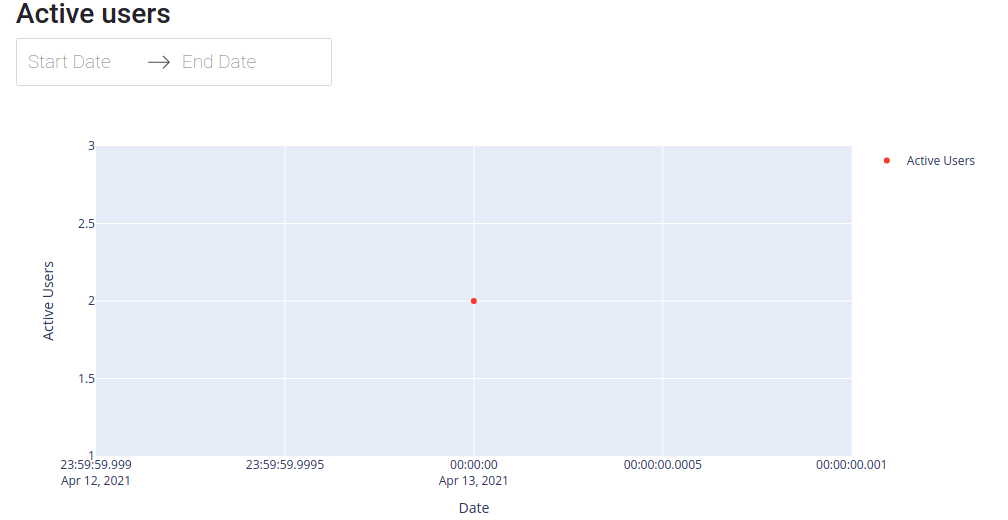
\includegraphics[width=16cm, keepaspectratio]{img/active.png}
    \caption{Gráfica de usuarios activos cada día}
    \label{fig:active}
\end{figure}

En todas las gráficas de Dash si se pone el cursor sobre uno de los puntos se puede ver la información con mayor detalle, como se muestra en la Figura \ref{fig:users}. Además, Dash añade varias opciones para interactuar con la gráfica, por ejemplo, se puede descargar la gráfica, hacer \textit{zoom} o seleccionar una parte de ella. \\
\subsection{Actividad en la plataforma}

La gráfica creada que se muestra en la Figura \ref{fig:sesion}, representa en el eje x el tiempo y en el eje y el número de sesiones, dando como resultado una gráfica de linea, con énfasis en los puntos para una mejor visualización. Esta gráfica muestra el número de sesiones por día. En la gráfica se observa que días ha habido más \textit{logins}, viéndose como en los meses de verano dicho número se ha reducido. Hace uso del índice \texttt{session\_log}, contando cuantas veces el campo \texttt{start\_date} se repite.\\



\begin{figure}[H]
    \centering
    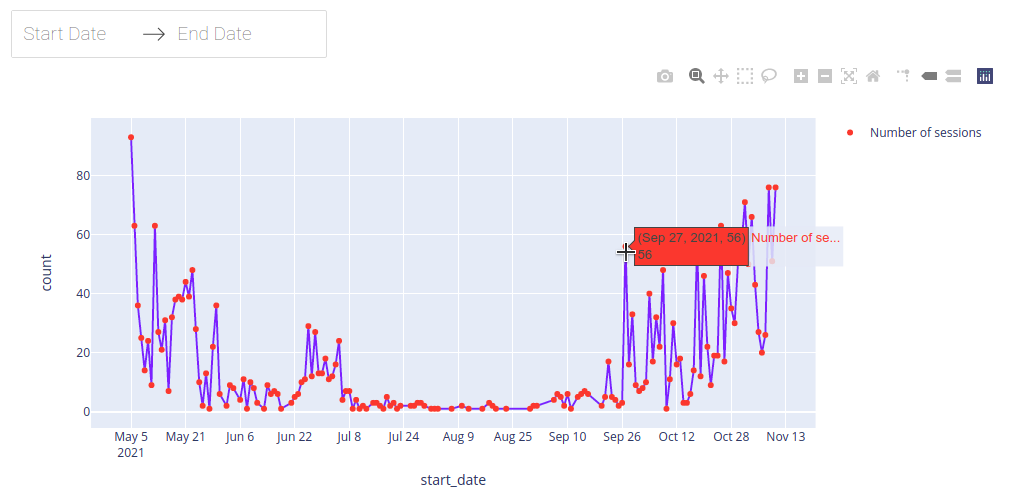
\includegraphics[width=16cm, keepaspectratio]{img/sesion.png}
    \caption{Gráfico sesiones totales por día}
    \label{fig:sesion}
\end{figure}
Se ha creado otra gráfica lineal de sesiones por día, pero en este caso solo se tiene en cuenta el número de sesiones por usuario único. La gráfica está creada de la misma manera que la gráfica del total de sesiones por día y con los mismos filtros (fechas y usuarios). Para que sean usuarios únicos, se ha eliminado los dataframes cuya columna de \texttt{username} se repetía. En la Figura \ref{fig:sesion_users}  se muestra una parte ampliada de dicha gráfica.\\

\begin{figure}[H]
    \centering
    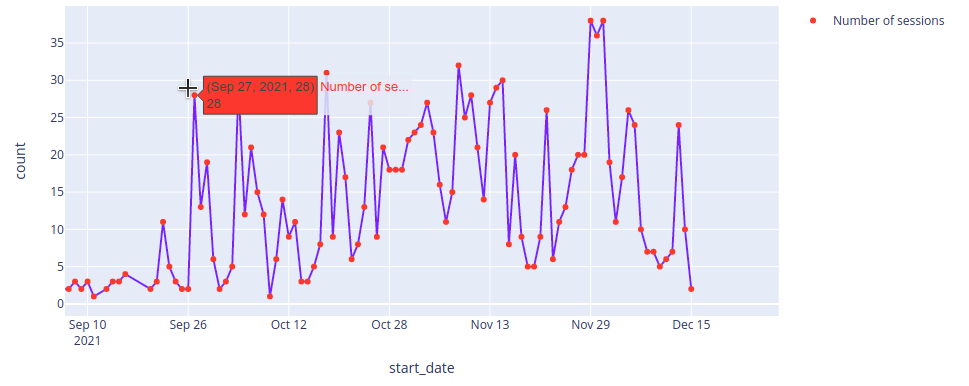
\includegraphics[width=16cm, keepaspectratio]{img/sesion_users.png}
    \caption{Gráfico sesiones únicas por día}
    \label{fig:sesion_users}
\end{figure}
La Figura \ref{fig:time} muestra una gráfica de barras en la cual se representa el tiempo mediante el eje x y la duración total de la sesión de los usuarios en minutos en el eje y. Además, se ha incluido una media que representa la duración media de las sesiones. Aquí podemos comprobar que a veces la media coincide con la duración total debido a que solo ha tenido que haber una sesión en ese día. Para realizar esta gráfica se ha utilizado los campos de \textit{duration} y \texttt{start\_date} del índice \texttt{session\_log}. Para crear la gráfica de barras junto con la gráfica de linea de la media, se utiliza el siguiente código:

\begin{verbatim}
def get_temporal_figure__session_time(df):
    fig = px.bar(df, x='start_date', y='duration')
    fig.add_trace(go.Scatter(x=df['start_date'], 
                              y=df['mean'], 
                              line=dict(color='red'), 
                              name='Mean'),
                  row=1, col=1)
    return fig
\end{verbatim}

\begin{figure}[H]
    \centering
    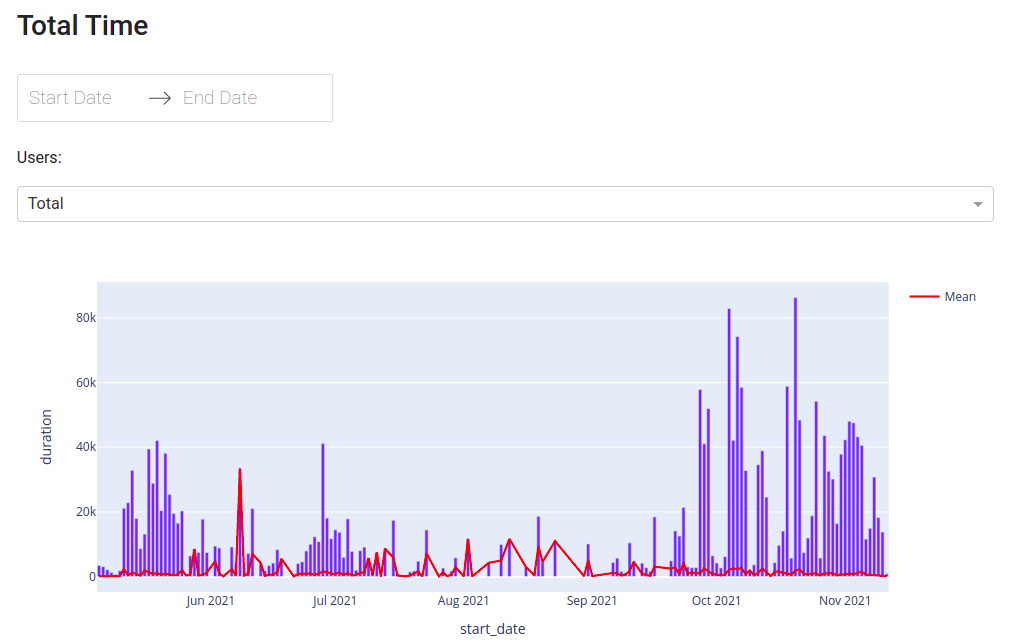
\includegraphics[width=16cm, keepaspectratio]{img/time.png}
    \caption{Gráfico de tiempo en Unibotics}
    \label{fig:time}
\end{figure}
Esta gráfica se puede filtrar tanto por fechas como por usuarios, pudiendo ver el tiempo dedicado de un usuario y la media total del tiempo que usa Unibotics dicho usuario, como se puede ver en la Figura \ref{fig:time_user}.

\begin{figure}[H]
    \centering
    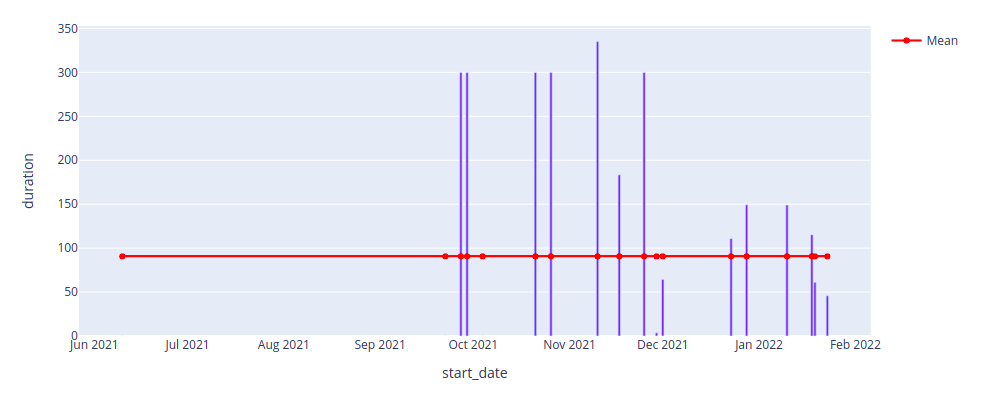
\includegraphics[width=14cm, keepaspectratio]{img/time_user.png}
    \caption{Gráfico de tiempo en Unibotics de un usuario}
    \label{fig:time_user}
\end{figure}

A fin de poder hacer un análisis de la media, la desviación típica o la moda se ha creado un histograma de las duraciones de las sesiones como se ve en la Figura \ref{fig:time_user}. En el eje x, se encuentran los diferentes intervalos de duraciones de los usuarios. En el eje y, representa cuantos usuarios han utilizado la plataforma durante el mismo tiempo. Para hacer el histograma de duración, se ha utilizado el código:
\begin{verbatim}
def get_temporal_figure__histogram_time(df):
    fig = px.histogram(df, x='duration')
    fig.update_layout(bargap=0.1)
return fig
\end{verbatim}

\begin{figure}[H]
    \centering
    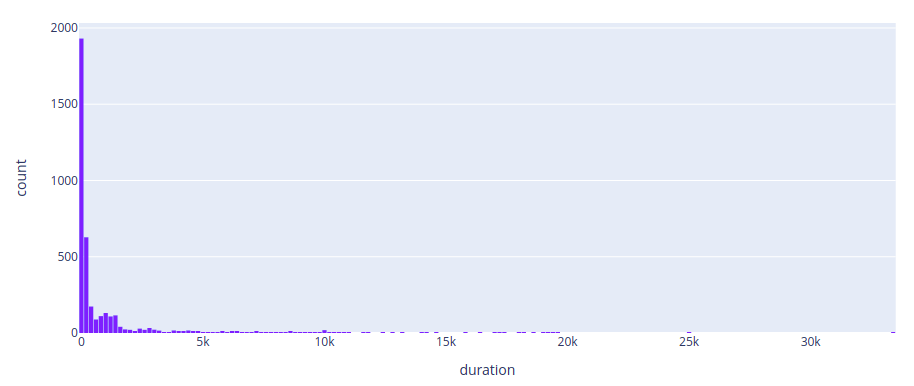
\includegraphics[width=15cm, keepaspectratio]{img/time_histogram.png}
    \caption{Histograma de las duraciones de sesiones}
    \label{fig:time_histogram}
\end{figure}
\newpage
En la siguiente gráfica que se ve en la Figura \ref{fig:activity} representa un mapa de calor con la actividad de los usuarios. Está dividido en cuadrados que representan cada día de un año, cuanto más intenso es el color verde más sesiones ha habido. Ha medida que disminuyen las sesiones la intensidad también baja. A parte del filtrado por fechas, tiene un filtro por usuario para ver la actividad por usuarios únicos o grupo de ellos. Como ocurría con la gráfica lineal de sesiones, el primer mapa de color cuenta el total de las sesiones y el segundo mapa de color cuenta las sesiones únicas por usuario. Las sesiones se han contado a través del campo de \textit{start\_date} del índice de \texttt{session\_log}.


\begin{figure}[H]
    \centering
    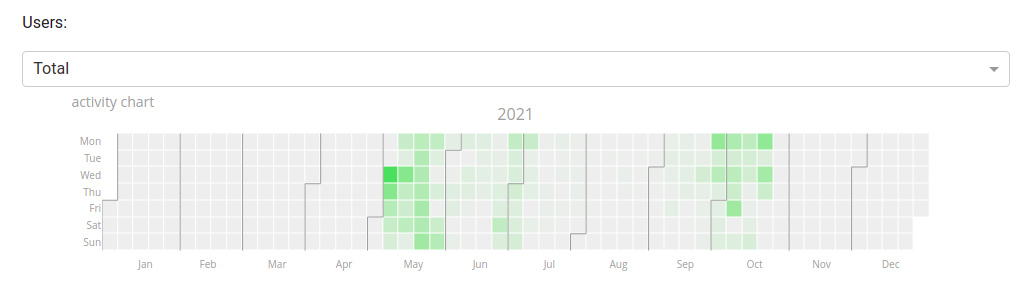
\includegraphics[width=17cm, keepaspectratio]{img/activity.png}
    \caption{Mapas de calor sesiones}
    \label{fig:activity}
\end{figure}
\newpage
En la Figura \ref{fig:mundo} se muestra un mapa geográfico con la localización de los usuarios que acceden a Unibotics. El tamaño de los puntos depende de la cantidad de sesiones, cuanto mayor sea el punto más sesiones hay. A la derecha se encuentra una leyenda con los países, se puede seleccionar uno o varios países en la leyenda para que solo se vean ellos en el mapa. Se puede filtrar por fechas. Para esta gráfica, se ha necesitado los campos de \textit{country}, \textit{continent} y \textit{alpha\_3} (código de los países), del índice de \texttt{session\_log}. Para hacer el mapa se necesita el siguiente código:
\begin{verbatim}
def get_temporal_figure__country(df):
    fig = px.scatter_geo(df, locations="alpha_3", color="country",
                     hover_name="country", size="count",
                     projection="natural earth")
return fig
\end{verbatim}


\begin{figure}[H]
    \centering
    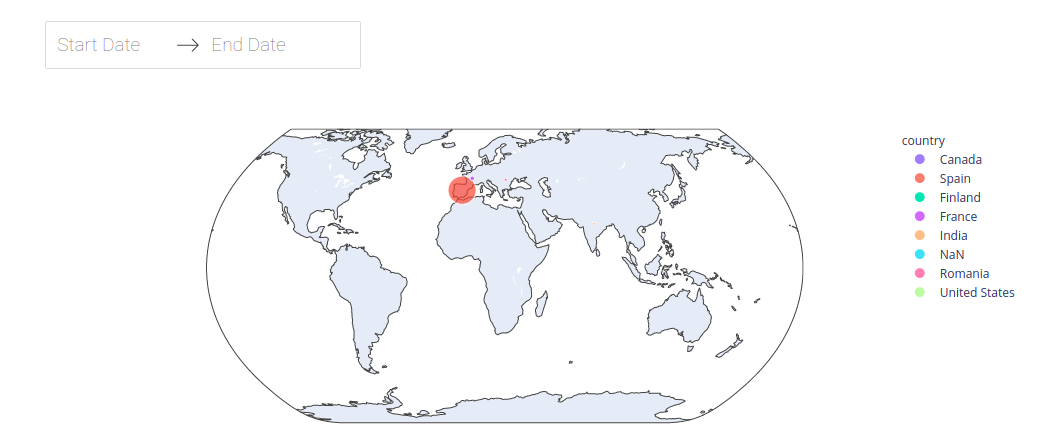
\includegraphics[width=17cm, keepaspectratio]{img/mundo.png}
    \caption{Mapa geográfico de sesiones}
    \label{fig:mundo}
\end{figure}
\newpage
Con el propósito de conocer el tiempo que invierten los usuarios en cada ejercicio se ha elaborado un histograma de las duraciones de los ejercicios. Esta gráfica dispone de un filtro del ejercicio que se desea comprobar, con el filtro de usuario y el de fechas. Por ejemplo, la Figura \ref{fig:histogram_exercise} es un histograma del ejercicio \textit{follow\_line}  de un grupo de usuarios y unas fechas concretas. Para realizar el histograma, se ha utilizado el índice de \texttt{exercises\_log}, en concreto los campos de \textit{exercise} y \textit{duration}.

\begin{figure}[H]
    \centering
    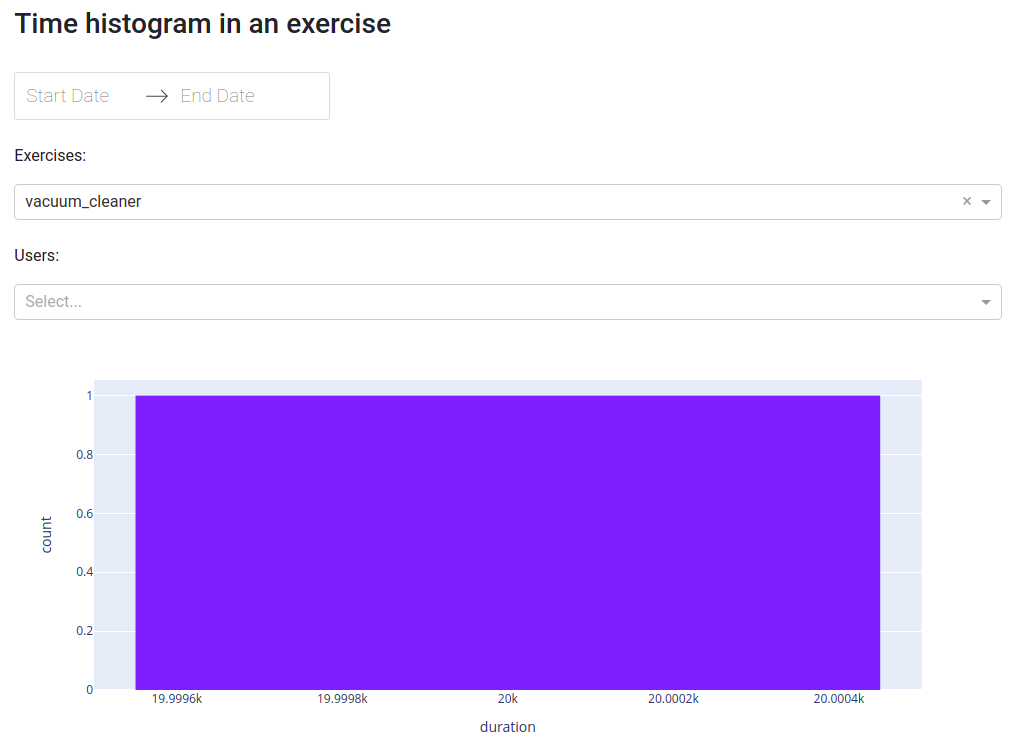
\includegraphics[width=17cm, keepaspectratio]{img/histogram_exercise.png}
    \caption{Histograma del ejercicio follow\_line de un grupo de usuarios }
    \label{fig:histogram_exercise}
\end{figure}
\newpage
\subsection{Acceso de los usuarios}
La Figura \ref{fig:browser} muestra una gráfica con los distintos navegadores que utilizan los usuarios para acceder a Unibotics, en formato porcentaje. En este caso se ve que una gran parte de inicio de sesiones es a través del navegador de Chrome. 


\begin{figure}[H]
    \centering
    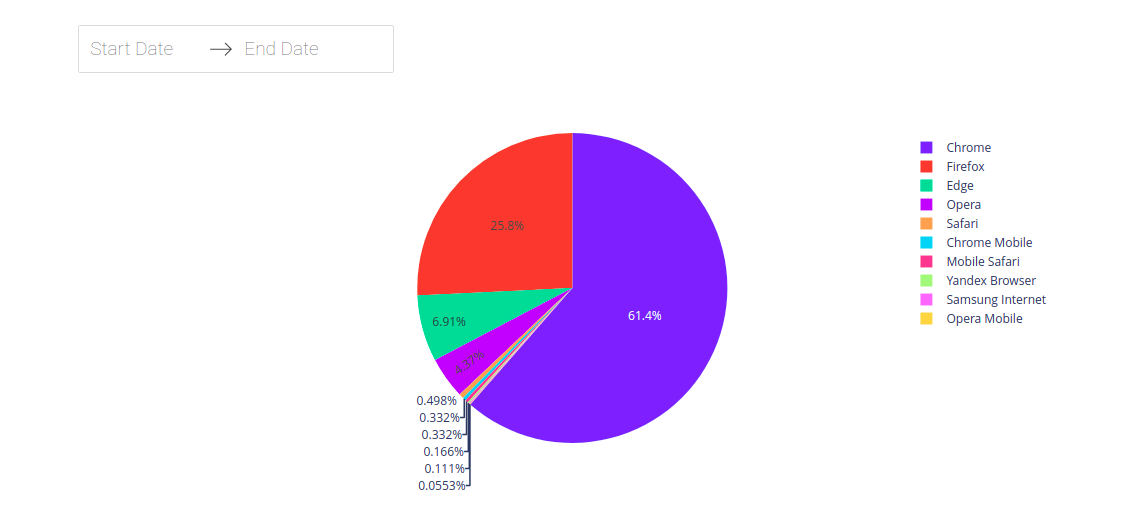
\includegraphics[width=18cm, keepaspectratio]{img/browser.png}
    \caption{Gráfico de navegadores}
    \label{fig:browser}
\end{figure}
Se ha creado una gráfica similar a la anterior para representar los Sistemas Operativos utilizados por los usuarios que acceden a Unibotics, como se puede ver en la Figura \ref{fig:os}. Ambas gráficas tienen filtro por fechas. En ambas gráficas circulares se ha hecho uso del campo \textit{browser} del índice de \texttt{session\_log}, el cual da la información sobre el sistema operativo y el navegador utilizado. Para realizar dichas gráficas circulares se programa el siguiente código:
\begin{verbatim}
def get_temporal_figure__browser(df):
    fig = px.pie(df, values='count', names='browser')
return fig
\end{verbatim}

\begin{figure}[H]
    \centering
    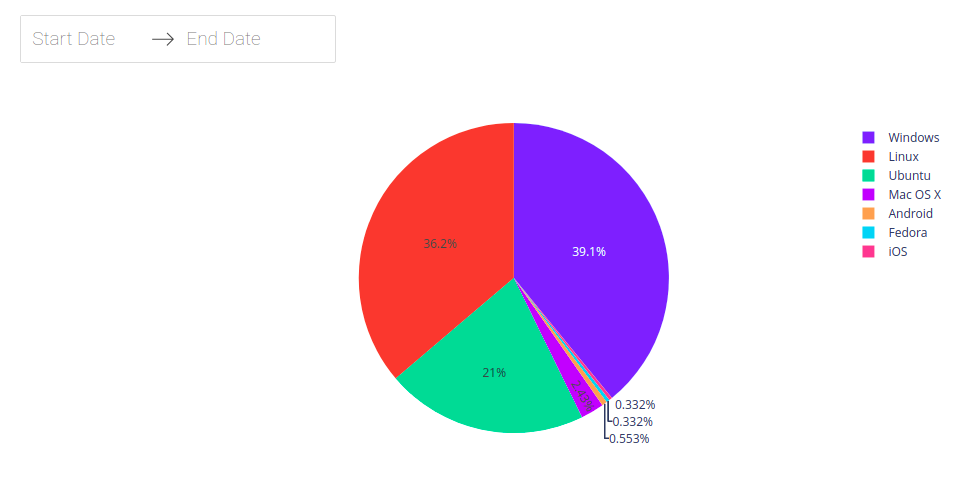
\includegraphics[width=15cm, keepaspectratio]{img/os.png}
    \caption{Gráfico de sistemas operativos}
    \label{fig:os}
\end{figure}
\subsection{Puntuaciones automáticas}
Las siguientes gráficas son las puntuaciones de estilo y eficacia que podrán ser vistas tanto por los usuarios (que pueden acceder a sus puntuaciones) como por los administradores (que pueden acceder a las puntuaciones de todos los usuarios).  Actualmente, las evaluaciones solo están disponibles en cuatro ejercicios. Se representa en una gráfica, en la que cada punto es una evaluación solicitada por el usuario. Las gráficas mostradas en las Figuras \ref{fig:score} y \ref{fig:score_efficacy}  son un ejemplo de las notas de estilo y eficacia de un usuario de la base de datos de prueba en el ejercicio \textit{follow\_line}. Las gráficas de los demás ejercicios son iguales. Para crear estas gráficas se utilizan todos los campos del índice de \texttt{style\_log} y \texttt{efficacy\_log}. El código de ambas gráficas es:
\begin{verbatim}
def score_fig(df):
    fig = px.scatter(df, x="date", y="score")
return fig
\end{verbatim}




\begin{figure}[H]
    \centering
    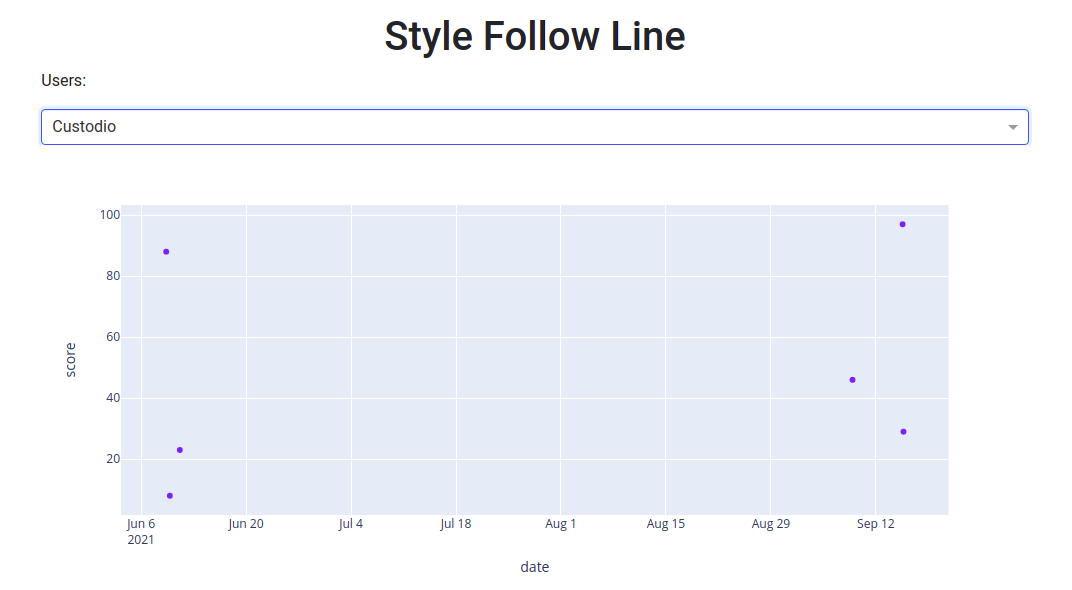
\includegraphics[width=17cm, keepaspectratio]{img/score.png}
    \caption{Gráfica de puntuación de estilo}
    \label{fig:score}
\end{figure}


\begin{figure}[H]
    \centering
    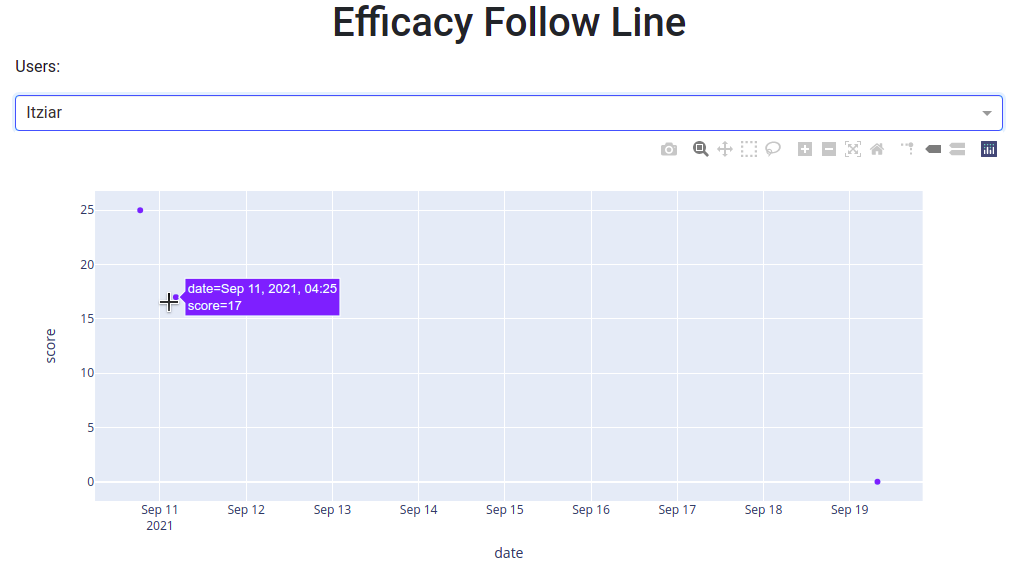
\includegraphics[width=17cm, keepaspectratio]{img/score_efficacy.png}
    \caption{Gráfica de puntuación de eficacia}
    \label{fig:score_efficacy}
\end{figure}






% CONCLUSIONES%
%%%%%%%%%%%%%%%%%%%%%%%%%%%%%%%%%%%%%%%%%%%%%%%%%%%%%%%%%%%%%%%%%%%%%%%%%%%%%%%%
\chapter{Conclusiones y trabajos futuros}\label{conclusión}

	En este último capítulo se detallan las conclusiones alcanzadas, así como las competencias adquiridas al realizar este TFG y los futuros trabajos que pueden extender la plataforma y las contribuciones actuales.
	
	\section{Conclusiones finales} 
	\label{sec:conclusiones_finales} 
El objetivo principal de este TFG se ha cumplido, ya que se ha conseguido integrar con éxito analíticas automáticas en Unibotics. Desde la propia herramienta se detecta el tipo de usuario que accede, de tal manera que es posible controlar y mostrar una visualización u otra dependiendo de este tipo de usuario. Analizando los subjetivos, mencionados en el capítulo 2, llegamos a las siguientes conclusiones:\\
\begin{itemize}
\item  El subjetivo 1 se ha realizado con éxito. Se ha podido capturar y guardar las interacciones de los usuarios en la plataforma. Las sondas que se han recogido, han sido: el inicio y fin de sesión de un usuario, entrada y salida de los ejercicios y las evaluaciones de eficacia y estilo del código de cada ejercicio. A través de código JavaScript, las sondas se capturan en el \textit{frontend} y se envían al servidor, el cual se encarga de grabarlas en la base de datos.
\newpage
\item  El subjetivo 2 se han conseguido con la utilización de la herramienta de Elasticsearch. El servidor web de Django es el encargado de grabar las sondas en la base de datos de Elasticsearch. Para conseguir guardar las sondas, se han creado cuatro índices, los cuales se explican en la subsección.

\item El subjetivo 3 se ha logrado con la integración de las visualizaciones de la información en el servidor web, gracias al entorno Dash. Ha permitido de una manera sencilla y potente la visualización de las sondas recogidas con Elasticserach. Estas gráficas representan una ventana de siete meses del uso de Unibotics de estudiantes reales. Ello ha permitido a los administradores comprender mejor el uso real de la plataforma. Se han añadido en varias gráficas el filtro de fecha y el filtro por usuario. Las primeras gráficas son las basadas en el número de registros y usuarios en la plataforma. Aquí, se encuentran tres gráficas lineales que representan los registros, los registros acumulados y los usuarios activos, cada día. El siguiente bloque de gráficas enseña la actividad en la plataforma. En él, se encuentran las gráficas de sesiones por día, tanto totales como por usuario único. Estas gráficas se pueden encontrar en formato lineal o en mapa de calor, como se describe en la subsección. También, está la gráfica del tiempo total empleado en la plataforma cada día y su histograma. Para ver la actividad en cada ejercicio, se ha creado un histograma de las duraciones en ellos, con los filtros mencionados en la subsección.  Y por último, la visualización de los metadatos, donde se hallan el sistema operativo y navegador que utilizan los usuarios para acceder a la plataforma.
\end{itemize}

	\section{Competencias adquiridas} 
	\label{sec:competencias_adquiridas} 
	Durante la realización del TFG he adquirido las siguientes competencias:
		
		\begin{itemize}
			\item Ampliado mis conocimientos sobre las tecnologías web, tanto el entorno de Django como HTML, CSS y JavaScript.
			
			\item Conocer cómo funciona una base de datos en un proyecto real, en el caso de MySQL, y saber desplegar e integrar una nueva base de datos no relacional, Elasticsearch. Comprender la importancia de la información para monitorizar un servicio web. 
			
			\item Entender las tecnologías de visualizaciones automáticas de la información gracias a Dash, la cual es una herramienta rápida y eficiente.
			
			\item Aprender a utilizar GitHub como repositorio donde desarrollar proyectos en equipo, haciendo uso de incidencias y parches. 
			
			\item Trabajar en una plataforma que está en continuo desarrollo, donde se han creado nuevas funcionalidades. Trabajar en equipo con otros desarrolladores de áreas diferentes a la trabajada en este proyecto.			
		\end{itemize}
	\section{Trabajos futuros} 
	\label{sec:trabajos_futuros} 

		En esta sección se proponen futuras líneas de trabajo para mejorar las analíticas automáticas:

		\begin{itemize}
\item Enriquecer las sondas que se encuentran en Unibotics añadiendo nuevas o añadiendo nuevos campos a los índices creados para recabar más información sobre el uso de la plataforma. Actualmente las sondas de puntuación de estilo y de eficacia solo se encuentran en cuatro ejercicios, así que se podrían añadir a los nuevos ejercicios que sean creados. Para recoger nuevas sondas será necesario la creación de nuevos índices en Elasticsearch y nuevas visualizaciones automáticas en la aplicación de Dash.
\item Incorporar a Elasticsearch medidas de rendimiento en el servidor web. El servidor está desplegado en \textit{Amazon Web Services} en producción por lo que se pueden añadir métricas de memoria ocupada o CPU consumida, entre otras. Luego se podrá correlar esas métricas con las sondas actuales, tales como el número de usuarios activos en la plataforma.
\item En este TFG se ha visualizado las sondas con los datos directamente recogidos, el siguiente paso que se podría hacer es correlacionar varias de las sondas recogidas y así enriquecer el conocimiento sobre el uso real que los estudiantes hacen de la plataforma y sobre los procesos de aprendizaje. Por ejemplo, saber si el tiempo en el que realizan un ejercicio afecta la nota obtenida en el ejercicio. Esto nos permite hacer análisis estadísticos o investigaciones científicas, como el efecto de la \textit{gamificación} en los procesos de aprendizaje.\\
		\end{itemize}

% BIBLIOGRAFÍA %
%%%%%%%%%%%%%%%%%%%%%%%%%%%%%%%%%%%%%%%%%%%%%%%%%%%%%%%%%%%%%%%%%%%%%%%%%%%%%%%%
\printbibliography

\end{document}